\documentclass[12pt,a4paper,twoside]{report}

\usepackage{graphicx}
\usepackage{setspace} % double spacing for text, single for captions, footnotes, etc.
%\usepackage{hypernat} % substitute for cite that allows hyperlinks
% \usepackage{natbib} % substitute for 'hypernat' that works on Windows.
\usepackage[sorting=none]{biblatex}
\usepackage[english]{babel}
\usepackage[utf8]{inputenc}
\usepackage{color}
\usepackage{hhline} % extended styles for tables
\usepackage{multirow}
\usepackage{makecell}
\usepackage{subfigure}
\usepackage{acronym}
\usepackage{hyperref}
\usepackage{caption} % figure links go to top of image
\usepackage{amsmath,amsmath,amssymb}
\usepackage{fancyhdr}
\usepackage{epsfig, amsmath}
\usepackage{algorithm}
\usepackage{algorithmic}
\usepackage{lipsum}
\usepackage[indent]{parskip}
\usepackage{dirtytalk}
\usepackage{appendix}
% general settings
\hypersetup{
linktocpage=true,
colorlinks=true,
linkcolor=blue,
citecolor=blue,
}
\definecolor{Hgray}{gray}{0.6}

\newenvironment{definition}[1][Definition]{\begin{trivlist}
\item[\hskip \labelsep {\bfseries #1}]}{\end{trivlist}}

\setlength{\topmargin}{0cm}
\setlength{\textheight}{23cm}
\setlength{\textwidth}{17cm}
\setlength{\oddsidemargin}{0cm}
\setlength{\evensidemargin}{0cm}
\setlength{\headheight}{1cm}

% indicates that 'sub-sub-sections' are numbered and appear in the index
\setcounter{secnumdepth}{3}
\setcounter{tocdepth}{3}

% settings for code
\renewcommand{\algorithmicrequire}{\textbf{Input:}}
\renewcommand{\algorithmicensure}{\textbf{Output:}}

\renewcommand\thesection{\thechapter.\arabic{section}}

% subsubsubsection
% \renewcommand\paragraph{\@startsection{paragraph}{4}{\z@}%
% % display heading, like subsubsection
%                                      {-3.25ex\@plus -1ex \@minus -.2ex}%
%                                      {1.5ex \@plus .2ex}%
%                                      {\normalfont\normalsize\bfseries}}

\addbibresource{refs/referencias.bib}

%%%%%%%%%%%%
% DOCUMENT %
%%%%%%%%%%%%
\begin{document}

% cover page
\newpage
\thispagestyle{empty}

\baselineskip 2em

%\vspace*{1cm}

\centerline{
\includegraphics[width=0.6\textwidth]{images/UOC-logo}}
\begin{center}
\textsc{Open University of Catalonia (UOC) \
Master's Degree in Data Science \
}

%\centerline {\pic{UOC}{4cm}}

\vspace*{1.5cm}

\textsc{\Large MASTER'S THESIS}

\vspace*{0.5cm}

\textsc{\large Area: 4}

%\textbf{\Huge VirtualTechLab Model: }

\vspace*{2.0cm}

\textbf{\Large Using Hierarchical Reinforcement Learning to reduce training costs in real-time strategy games}

% \textbf{\large xxx subtitle (if any) xxx}

\vspace{2.5cm}
\baselineskip 1em

\baselineskip 2em
-----------------------------------------------------------------------------\\
Author: David Pérez Gómez\\
Tutor: Luis Esteve Elfau\\
Professor: Ismael Benito Altamirano\\
-----------------------------------------------------------------------------\\
\vspace*{1.5cm}
Barcelona, \today

\end{center}

\newpage
\pagestyle{empty}
\hfill
\newpage
\pagenumbering{roman}
\setcounter{page}{1}
\pagestyle{plain}
%%%%%%%%%%%%%%%%
%%% CREDITS %%%
%%%%%%%%%%%%%%%%
\chapter*{Credits/Copyright}

\vspace{1cm}

\begin{figure}[ht]
\centering

\includegraphics[scale=1]{images/license.png}
\end{figure}

Attribution-NonCommercial-NoDerivs 3.0 Spain (CC BY-NC-ND 3.0 ES) 

\href{https://creativecommons.org/licenses/by-nc-nd/3.0/es/}{3.0 Spain of CreativeCommons}.
%%%%%%%%%%%%%
%%% RECORD %%%
%%%%%%%%%%%%%
\chapter*{FINAL PROJECT RECORD}

\begin{table}[ht]
\centering{}
\renewcommand{\arraystretch}{2}
\begin{tabular}{r | l}
\hline
Title of the project: & \makecell[cl]{Using Feudal Reinforcement Learning to\\reduce training costs in real-time strategy games}\\
\hline
Author's name: & David Pérez Gómez\\
\hline
Collaborating teacher's name: & Luis Esteve Elfau\\
\hline
PRA's name: & Ismael Benito Altamirano\\
\hline
Delivery date (mm/yyyy): & 01/2025\\
\hline
Degree or program: & Máster Universitario en Ciencia de Datos\\
\hline
Final Project area: & Area 4\\
\hline
Language of the project: & English\\
\hline
Keywords & \makecell[cl]{Machine Learning,\\ Deep Reinforcement Learning,\\ Feudal Reinforcement Learning,\\ Efficiency, Emissions, StarCraft II,\\ Real-time Strategy}\\
\hline
\end{tabular}
\end{table}
% %%%%%%%%%%%%%%%%%%%
%%% DEDICATION %%%
%%%%%%%%%%%%%%%%%%%
\chapter*{Dedication/Quote}

Brief words of dedication and/or a quote.
% %%%%%%%%%%%%%%%%%%%
%%% Acknowledgements %%%
%%%%%%%%%%%%%%%%%%%
\chapter*{Acknowledgements}

If deemed appropriate, mention the people, companies or institutions that have contributed to the realization of this project.
\onehalfspacing
%%%%%%%%%%%%%%%%
%%% ABSTRACT %%%
%%%%%%%%%%%%%%%%
\chapter*{Abstract}
\addcontentsline{toc}{chapter}{Abstract}

The growing interest in AI research has led to a massive increase in model sizes and compute costs of their training over the last several years. With the current concerns about climate change and the necessity of reducing carbon emissions, finding ways to minimize the environmental impact of the AI industry is more important than ever.

The object of this study is to find evidence that a hierarchical approach to deep reinforcement learning can be used to reduce the costs of training agents in complex environments while maintaining the final agent performance. For this purpose, we use StarCraft II as the training environment: a popular real-time strategy game that affords a massive action space and is easy to use for reinforcement learning experiments thanks to the library PySC2.

\vspace{1.5cm}

\textbf{Keywords}: Deep Reinforcement Learning, Hierarchical Reinforcement Learning, Efficiency, Emissions, StarCraft II
%%%%%%%%%%%%%%%%
%%% ABSTRACT %%%
%%%%%%%%%%%%%%%%
\chapter*{Resumen}
\addcontentsline{toc}{chapter}{Resumen}

El creciente interés en la investigación de IA ha dado lugar a un enorme aumento en el tamaño de los modelos y en el coste computacional de su entrenamiento a lo largo de los últimos años. Dada la preocupación actual por el cambio climático y la necesidad de reducir emisiones de carbono, hallar formas de minimizar el impacto que la industria de la IA tiene sobre el medio ambiente es más importante que nunca.

El objetivo de este estudio es encontrar evidencias de que se puede utilizar un enfoque jerárquico en el aprendizaje por refuerzo profundo para reducir los costes de entrenamiento de agentes en entornos complejos al mismo tiempo que se mantiene el nivel de rendimiento del agente final. Para este fin, utilizamos StarCraft II como entorno de entrenamiento: un juego de estrategia en tiempo real que proporciona un enorme espacio de acciones y es fácil de utilizar para aprendizaje por refuerzo gracias a una librería existente.

\vspace{1.5cm}

\textbf{Keywords}: Aprendizaje Autormático, Aprendizale por Refuerzo Profundo, Aprendizale por Refuerzo Feudal, Eficiencia, Emisiones, StarCraft II, Estrategia en Tiempo Real
% %%%%%%%%%%%%%%%%
%%% ABSTRACT %%%
%%%%%%%%%%%%%%%%
\chapter*{Resum}
\addcontentsline{toc}{chapter}{Resum}

Text with a summary of the project, that is, a concise explanation of the project/problem addressed, its objectives/resolution methods, and the results and conclusions (it cannot be a list, but rather a continuous text written in a structured way). If a reference is necessary in this text, it will be noted at the bottom of the same page. In this section, a more literary and colloquial language can be used than for the rest of the document.

The Abstract will be written twice. One version must be \textbf{obligatorily in English}. The other version must be written in Catalan or Spanish. If the rest of the document is not written in English, it will be necessary to write the second version of the Abstract in the language used for the rest of the report. The word Abstract will be changed to \textbf{Resum}'' or \textbf{Resumen}'' in the Catalan and Spanish versions, respectively.

Recommended length: maximum 250 words.

How to write a good Abstract:

\href{http://www.ece.cmu.edu/~koopman/essays/abstract.html}{http://www.ece.cmu.edu/~koopman/essays/abstract.html}

\vspace{1.5cm}

\textbf{Keywords}: Keywords related to the project separated by commas. For example, for this document, they could be Model, Guideline, Template, Report, Bachelor's/Master's Thesis.
\newpage

\pagestyle{fancy}
\renewcommand{\chaptermark}[1]{ \markboth{#1}{}}
\renewcommand{\sectionmark}[1]{\markright{ \thesection.\ #1}}
\lhead[\fancyplain{}{\bfseries\thepage}]{\fancyplain{}{\bfseries\rightmark}}
\rhead[\fancyplain{}{\bfseries\leftmark}]{\fancyplain{}{\bfseries\thepage}}
\cfoot{}

% table of contents
\cleardoublepage
\phantomsection
\addcontentsline{toc}{chapter}{Table of Contents}
\tableofcontents
% list of figures
\cleardoublepage
\phantomsection
\addcontentsline{toc}{chapter}{List of Figures}
\listoffigures
% list of tables
\cleardoublepage
\phantomsection
\addcontentsline{toc}{chapter}{List of Tables}
\listoftables

\thispagestyle{empty}

\pagenumbering{arabic}

% chapters of the document

\chapter{Introduction}
\label{chapter:introduction}

\section{Overview of the problem}

In recent years, interest in the field of artificial intelligence has boomed, both among the public and among researchers. In 2022, the number of publications related to AI was nearly triple that of ten years prior \cite{Nestor:2024}. However, most of this research appears to focus mainly on the accuracy of the AI models, with only a small percentage of papers being dedicated to or giving similar importance to their efficiency \cite{Schwartz:2019}.

By 2018, the computing cost of some of the biggest deep learning models had increased by a factor of over 3.000.000 compared to six years before \cite{Amodei:2018}, and the doubling period for that cost is still estimated to be less than a year \cite{Jaime:2022}. When considering that the energy consumed often comes from non-renewable and carbon-positive sources \cite{Strubell:2019}, the impact that the industry has on the environment cannot be overlooked.

In the case of reinforcement learning, one of the biggest factors that increases the training costs is the complexity of the environment that the model has to learn. As the number of possible states and actions increases, and especially if the results of the actions are non-deterministic or there are other elements outside of the agent's control that can affect the environment, the difficulty of training and tuning RL models skyrockets. A potential solution to that problem can be found in hierarchical reinforcement learning, a methodology that consists of subdividing the main goal of the environment into several subtasks and training smaller specialized agents for each of the tasks \cite{Barto:2003, Al-Emran:2015, Pateria:2021}. Our hypothesis is that this approach can be used in complex environments to achieve solutions with equal or greater performance than traditional reinforcement learning with a smaller compute cost, which translates into less energy consumption and less carbon emissions.

\section{Personal motivation}

My particular motivation to work on this project is twofold. On one hand, and like many people, I am quite concerned about the current trend of global warming and the grim outlook for the environment in the coming decades. As such, taking part in a project aimed at finding solutions to reduce carbon emissions aligns strongly with my values.

On the other hand, I see this as an opportunity to further study and learn about the topic of reinforcement learning. I was already very interested in RL before beginning my studies in this Master's course, and that interest has only grown as I have learned more about the topic. For this project, I am excited to work on hierarchical reinforcement learning as a particular branch of the broader discipline.

\section{Goals}
\label{section:goals}

In this thesis, we will continue the work of prior students \cite{Caceres:2024, Gimenez:2024} in determining whether a hierarchical assembly of specialized agents can be used to achieve comparable results to a single agent while generating less carbon emissions during training. In the previous work, it was established that the multi-agent strategy was able to achieve better performance and greater consistency than the single agent, but not with a smaller energy consumption.

The main goal of the project will be to find under what conditions a multi-agent strategy can outperform a single agent in both performance and training efficiency. The following is the list of subgoals we have chosen that will help us reach the main goal:

\begin{itemize}
    \item \textbf{Reducing built-in logic in actions.} In the previous environment, actions had a considerable amount of pre-programmed logic to simplify and streamline the action space. We believe this might have allowed a single agent, and even a random agent, to compete more closely with the hierarchical agent, which should fair better with a more complex action space.
    \item \textbf{Improving the reward signal.} We believe there is still room to improve when it comes to the default reward signal provided by the environment and the custom reward used in the previous work.
    \item \textbf{Finding new subtasks.} The strength of the hierarchical strategy rests in dividing the main objective of the environment into different subtasks in which to train each of the specialized agents. Finding additional ways to divide the action space may prove beneficial for the efficiency of the multi-agent.
\end{itemize}

\section{Sustainability, diversity, and ethical/social challenges}

Before starting the project, we have assessed its impact in the various dimensions of the Ethical and Global Commitment Competency.

\subsection{Sustainability}

This project aims to discover ways to reduce energy consumption and carbon emissions during the training of deep reinforcement learning agents. If we are successful, it could lead to a modest but positive impact on the environmental footprint of future research and development. As such, it aligns with Goal 13 \cite{UN:Goal13} of the UN Sustainable Development Goals (SDG).

\subsection{Ethical behavior and social responsibility}

The technical nature of this project means it is unlikely to have any direct impact in ethical or social aspects. Additionally, since we don't make use of any data obtained from people, there is no risk of improper use of personal data.

\subsection{Diversity, gender and human rights}

Similarly, the goals of the project would not have any positive or negative impact on matters of diversity, gender, or human rights. The lack of human-generated data also minimizes the risk of introducing biases based on human characteristics.

\section{Approach and methodology}

\subsection{Development methodology}

For this project, we will take an agile approach to development, working on incremental tasks according to our goals. This will allow us to experiment iteratively with different solutions and to remain flexible and course-correct in accordance with our findings and the needs of the project.

\subsection{Tools}
\label{section:tools}

Given the access to the previous work, we will continue using the same technical setup and tooling:

\begin{itemize}
    \item For the environment that the agents will be trained, we will use the real-time strategy game StarCraft II\footnote{\url{https://www.starcraft2.com/}} by Blizzard Entertainment, Inc\footnote{\url{https://www.blizzard.com/}}.
    \item The project will be developed in Python\footnote{\url{https://www.python.org/}}.
    \item We will use the library PyTorch\footnote{\url{https://pytorch.org/}} for much of the general machine learning logic.
    \item To interact with the environment, we will use PySC2 \cite{Vinyals:2017}, a library that facilitates using StarCraft II as a machine learning environment by allowing access to the game's API and providing other utilities such as mini-games and custom maps.
\end{itemize} 

\section{Project planning}

This project will take place over a period of around 18 weeks. As illustrated in figure \ref{fig:gantt}, the planning for the project has been organized in three main tasks, each with their own subtasks, as follows:

\begin{figure}[!h]
    \centering
    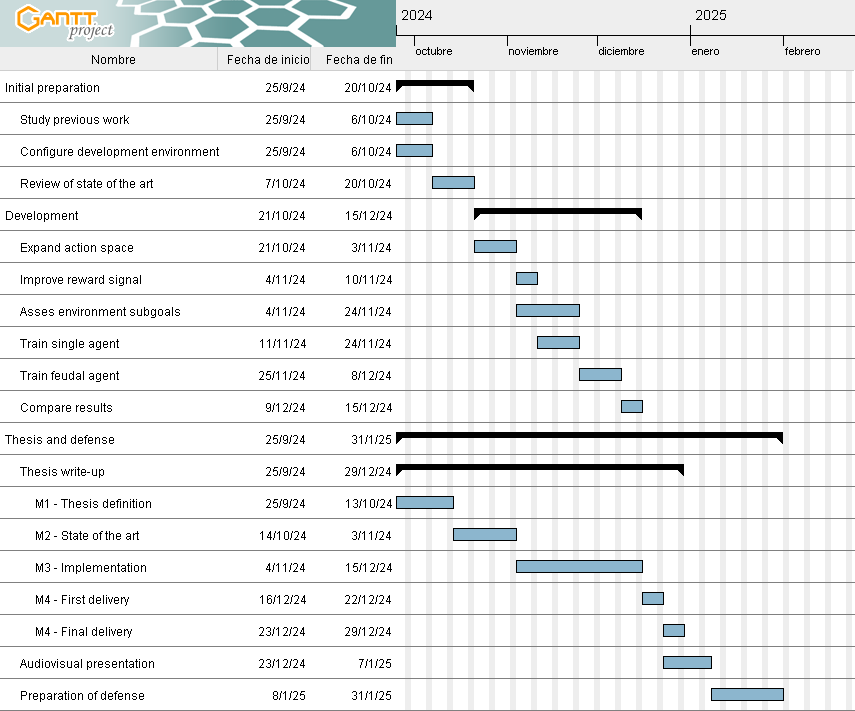
\includegraphics[width=.9\textwidth]{figs/TFM_Gannt.png}
    \caption[Gantt diagram of the planning for this project]{Gantt diagram of the planning for this project. Created with GanttProject\protect\footnotemark.}
    \label{fig:gantt}
\end{figure}
\footnotetext{\url{https://www.ganttproject.biz/}}

\begin{description}
    \item[Initial preparation] The first step of the project will involve studying and becoming familiar with the existing work that we will be using as a base, as well as setting up the development environment, which includes the tools mentioned in section \ref{section:tools}. Additionally, we will review the state of the art on relevant topics, such as hierarchical and feudal reinforcement learning.
    \item[Development] The development phase will take up most of the available time for the project. This is where we will try to achieve the goals laid out in section \ref{section:goals}. First will come the changes to the environment: the expansion of the action space and the improvement to the reward signal. After that, we will begin training the single agent to use as a benchmark. At the same time, we will study the environment in search of new subgoals. Finally, we will train the feudal agents and will compare the results of both strategies.
    \item[Thesis and defense] The process of writing the thesis document will be carried out in parallel to the development of the project and will follow a schedule of mandatory handouts---M1 to M5. Once the document is finished, we will move on to prepare the audiovisual presentation and the final defense.
\end{description}

\section{Report structure}

Next, we include a brief description of the future chapters of this report:

\begin{description}
    \item[Chapter \ref{chapter:state_of_the_art}] Presents an introduction to reinforcement learning and the state of the art of the techniques that we will use throughout the project.
    % TODO Complete
\end{description}
\chapter{State of the art}
\label{chapter:state_of_the_art}

In this chapter, we introduce the basic elements and concepts of reinforcement learning, we describe the structure of a reinforcement learning problem, the solutions that are relevant to this project and the concept of hierarchical reinforcement learning, and finally, we review the state of the art on the matter of efficiency in the field of reinforcement learning.

\section{Introduction to reinforcement learning}

Reinforcement learning (RL) is a form of machine learning that can be described as \say{a way of programming agents by reward and punishment without needing to specify how the task is to be achieved} \cite{Kaelbling:1996}. The goal of reinforcement learning is to produce an agent capable of solving a particular problem within an environment. However, the agent has no initial knowledge of the task that it must complete or the effect that its actions have. Instead, it must learn through trial and error by interacting with the environment.

\subsection{Elements}

There are four core elements in a reinforcement learning problem:

\begin{description}
    \item[Agent] The program that makes decisions and takes actions. It must learn what is the best course of action through its experience interacting with the environment.
    \item[Environment] The context that houses the problem to be solved.
    \item[States] Snapshots that describe of the environment at a particular point in time and that the agent uses to make its decisions.
    \item[Reward signal] Real scalar magnitude that the agent needs to maximize in order to achieve its goal.
\end{description}

These elements are described in greater detail below.

\subsubsection{Environment}

\begin{figure}[!h]
    \centering
    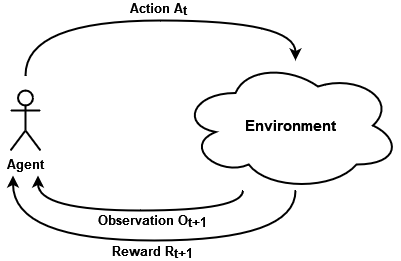
\includegraphics[width=.5\textwidth]{figs/RL_schema.png}
    \caption{Agent-Environment interaction}
    \label{fig:interaction}
\end{figure}

The environment encompasses all that is external to the agent. The agent learns by interacting with the environment in a series of discreet instants, or time steps, as depicted in figure \ref{fig:interaction}. On any given step $t$, the agent:

\begin{enumerate}
    \item receives an observation of the environment $O_t$,
    \item receives a reward $R_t$ based on the current state of the environment, and
    \item executes an action $A_t$.
\end{enumerate}

In response, the environment:

\begin{enumerate}
    \item receives the action $A_t$,
    \item generates a new observation of the environment $O_{t+1}$, and
    \item emits a new reward $R_{t+1}$.
\end{enumerate}

\subsubsection{States}

The states describe the evolution of the environment to reflect the actions taken by the agent. For every time step $t$, the state $S_t$ contains the information of all previous observations, actions and rewards, and can be used to determine how the environment will change in the next time step. Depending on the design of the environment and the agent, the agent may not have perfect knowledge of the sate, meaning that the observation $O_t$ it receives does not equal the true state $S_t$. These environments are called partially observable, as opposed to fully observable environments, in which $O_t = S_t$.

\subsubsection{Reward signal}

The reward signal $R_t$ is a real scalar value that the agent receives after every action it takes. On any given time step $t$, the sum of all future rewards is a random variable $G_t$ known as \textit{return}. The \textit{reward hypothesis} sates that the solution to any problem can be thought as the maximization of the expected value of the return \cite{Sutton:2018}. As such, the agent's goal is to learn actions that maximize the return at the end of the scenario, which doesn't necessarily mean maximizing the immediate reward for the current state. Sometimes it may be necessary to forgo a large immediate reward in favour of greater long-term return.

\begin{equation}
    G_t = R_{t+1} + R_{t+2} + R_{t+3} + \ldots
\end{equation}

Depending on the nature of the environment, it may be the case that the number of steps isn't finite. This could mean that the return never converges. To solve this, a discount value $\gamma \in [0,1]$ is introduced, which reduces the weight of rewards the further away they are from the current time step.

\begin{equation}
    G_t = R_{t+1} + \gamma R_{t+2} + \gamma^2 R_{t+3} + \ldots
\end{equation}

The return can also be expressed recursively:

\begin{align}
\begin{split}
    G_t = &R_{t+1} + \gamma R_{t+2} + \gamma^2 R_{t+3}  + \gamma^3 R_{t+4} + \ldots\\
    &R_{t+1} + \gamma(R_{t+2} + \gamma R_{t+3} + \gamma^2 R_{t+4} + \ldots)\\
    &R_{t+1} + \gamma G_{t+1}
\end{split}
\end{align}

\subsubsection{Agent}

While the previous three elements describe the problem, the agent represents the solution. It is comprised of one or more of the following elements.

\subsubsection*{Policy}

The policy $\pi(\cdot)$ is a function that determines the action that the agent will take in any particular state. There are two types of policies:

\begin{itemize}
    \item \textbf{Deterministic:} The policy maps a single action to each state, meaning that the agent will always take action $a$ when in the state $s$.
    \begin{equation}
        a = \pi(s)
    \end{equation}
    \item \textbf{Stochastic:} The policy assigns one or more actions following a probability distribution to each state. In this case, the policy $\pi(a|s)$ represents the probability that action $a$ will be taken when in the state $s$.
    \begin{equation}
        \pi(a|s) = P(A_t=a|S_t=s)
    \end{equation}
\end{itemize}

\subsubsection*{Value function}

The value function calculates the expected accumulated future reward (the return) of a state given a policy to follow. This allows us to estimate how \say{good} it is to be in any specific state. There are two approaches:

\begin{itemize}
    \item \textbf{State value function:} It calculates the expected return of following the policy $\pi$ from the state $s$.
    \begin{align}
    \begin{split}
        v_\pi(s) &= \mathbb{E}_\pi[G_t|S_t = s]%\\
        % &= \mathbb{E}_\pi[R_{t+1} + \gamma R_{t+2} + \gamma^2R_{t+3} + \ldots|S_t = s]\\
        % &= \mathbb{E}_\pi[R_{t+1} + \gamma G_{t+1}|S_t = s]
    \end{split}
    \end{align}
    \item \textbf{Action value function:} It calculates the expected return of taking the action $a$ (regardless of policy) in the state $s$ and then following the policy $\pi$.
    \begin{align}
    \begin{split}
        q_\pi(s,a) &= \mathbb{E}_\pi[G_t |S_t = s,A_t = a]%\\
        % &= \mathbb{E}_\pi[R_{t+1} + \gamma R_{t+2} + \gamma^2R_{t+3} + \ldots|S_t = s,A_t = a]\\
        % &= \mathbb{E}_\pi[R_{t+1} + \gamma G_{t+1}|S_t = s,A_t = a]
    \end{split}
    \end{align}
\end{itemize}

\subsubsection*{Model}

The model is an internal representation of the environment that the agent uses to try to predict how it will behave. It is an optional element, and agents may or may not have internal models. These models can be of two types:

\begin{itemize}
    \item \textbf{Transition model $\mathcal{P}$:} It estimates, given the current state $s$ and the action to take $a$, the next state $s^\prime$ that the environment will generate.
    \begin{equation}
        \mathcal{P}^a_{ss^\prime} = p(s^\prime|s,a) \approx P(S_{t+1} = s^\prime|S_t = s, A_t = a)
    \end{equation}
    \item \textbf{Reward model $\mathcal{R}$:} It approximates the expected reward that the agent will receive when performing the action $a$ in the state $s$.
    \begin{equation}
        \mathcal{R}^a_s = r(s,a) \approx \mathbb{E}[R_{t+1}| S_t = s, A_t = a]
    \end{equation}
\end{itemize}

\subsection{Agent taxonomy}

There are two main axes to classify agents based on what elements they contain.

\subsubsection*{Value function and policy}

An agent can be one of three types depending on whether it makes use of a value function or a policy to determine its actions:

\begin{itemize}
    \item \textbf{Based in value function.} The value function is explicit and the policy is implicit.
    \item \textbf{Based in policy.} The policy is explicit and the value function is implicit.
    \item \textbf{Actor-Critic.} Both the value function and the policy are explicit.
\end{itemize}

\subsubsection*{Model}

There are two types of agents based on the use, or lack thereof, of an internal model:

\begin{itemize}
    \item \textbf{Model free.} The agent does not contain a model of the environment and it doesn't try to learn its dynamics.
    \item \textbf{Model based.} The agent does contain a model of the environment and it first tries to learn its dynamics to later make predictions based on them.
\end{itemize}

\subsection{Challenges in reinforcement learning}
\label{sec:challenges}

Next, we introduce some of the common challenges that are found in RL.

\subsubsection*{Learning and planning}

There are two main configuration of sequential decision-making problems. The first is reinforcement learning in the strict sense, where the environment is unknown to the agent, which must interact with it and improve its policy by trial and error. In the second, planning, the agent starts with a perfect model of the environment and uses it to calculate improvements to the policy.

% These approaches a usually separated, but they may sometimes be related, for example in problems where reinforcement learning is used to create a model of the environment which is then used in planning.

\subsubsection*{Exploration and exploitation}

Exploration is the process by which the agent finds new paths or alternative courses of action that allow it to discover better solutions. Exploitation is the process of using the best known solutions to maximize the reward. As such, there is a balance to be found between the two, since both are necessary to solve the problem: the agent should work on optimizing the most promising solutions, but also keep exploring alternatives.

\subsubsection*{Prediction and control}

A prediction is the concept of evaluating the future based on a policy $\pi$, such as predicting the return with a value function $v_\pi(s)$. Control refers to optimizing the future, for example, by finding the optimal policy $\pi_\ast(s)$ that would generate the greatest return. These concepts are related as follows:

\begin{equation}
    \pi_\ast(s) = \underset{\pi}{\operatorname{argmax}}\,v_\pi(s)
\end{equation}

The optimal policy is the one that results in the maximum value function. Typically, in reinforcement learning problems, is necessary to first solve the prediction problem by estimating $v_\pi(s)$ in order to solve the control problem, since the value function is used to evaluate and compare different policies.

\section{Definition of the problem}

A reinforcement learning problem can be described as a Markov decision process \cite{Sutton:2018}, which is defined by the tuple $<\mathcal{S}, \mathcal{A},\mathcal{P},\mathcal{R},\gamma>$.

\begin{description}
    \item[$\mathcal{S}$] is the finite set of all possible states in the environment ($S_t \in \mathcal{S}$). These states follow the \textit{Markov property} (equation \ref{eq:markov}), which means that the evolution of a state depends only on that state, and is independent of all the previous ones \cite{Sutton:2018}.
    \begin{equation}
    \label{eq:markov}
        P(S_{t+1}|S_t) = P(S_{t+1}|S_1, S_2, \ldots, S_t)
    \end{equation}
    \item[$\mathcal{A}$] is the finite set of all possible actions that the agent can take ($A_t \in \mathcal{A}$).
    \item[$\mathcal{R}$] is the finite set of all possible rewards ($R_t \in \mathcal{R}$). 
    \item[$\mathcal{P}$] is the state transition matrix, which contains the probabilities for all the transition from a state $s$ to the next state $s^\prime$. Its elements can be of one of two forms, depending on whether the reward for the transition is deterministic (equation \ref{eq:transition_det}) or stochastic (equation \ref{eq:transition_sto}).
    \begin{equation}
    \label{eq:transition_det}
        p(s^\prime|s, a) = P(S_{t+1} = s^\prime|S_t = s, A_t = a)
    \end{equation}
    \begin{equation}
    \label{eq:transition_sto}
        p(s^\prime, r|s, a) = P(S_{t+1} = s^\prime, R_{t+1} = r|S_t = s, A_t = a)
    \end{equation}
    \item[$\gamma$] is the discount value applied to the rewards when calculating the return.
\end{description}

% Once these elements are defined, the expected value of the rewards used by the value functions can be calculated.

% \begin{align}
% \begin{split}
%     \label{eq:bellman_state}
%     v_\pi(s) &= \mathbb{E}_\pi[R_{t+1} + \gamma G_{t+1}|S_t = s] \\
%     &= \sum_{\forall a \in \mathcal{A}}{\pi(a|s)} \sum_{\substack{\forall r \in \mathcal{R} \\ \forall s^\prime \in \mathcal{S}}}{p(r,s^\prime|s,a)[r + \gamma v_\pi(s^\prime)]}
% \end{split}
% \end{align}

% \begin{align}
% \begin{split}
%     \label{eq:bellman_action}
%     q_\pi(s,a) &= \mathbb{E}_\pi[R_{t+1} + \gamma G_{t+1}|S_t = s, A_t = a] \\
%     &= \sum_{\substack{\forall r \in \mathcal{R} \\ \forall s^\prime \in \mathcal{S}}}{p(r,s^\prime|s,a)[r + \gamma \sum_{\forall a \in \mathcal{A}}{\pi(a^\prime|s^\prime)q_\pi(s^\prime,a^\prime)}]}
% \end{split}
% \end{align}

\section{Solutions}

To solve a reinforcement learning problem it is necessary to find the optimal state value function $v_\ast(s)$ and optimal action value function $q_\ast(s,a)$. These are the value functions that return the greatest value from all policies.

\begin{equation}
    v_\ast(s) = \max_{\pi}{v_\pi(s)}
\end{equation}

\begin{equation}
    q_\ast(s,a) = \max_{\pi}{q_\pi(s,a)}
\end{equation}

These functions are related in that the optimal state value function of a state $s$ will be equal to the optimal action value function when selecting the action $a$ that maximizes the return in that state.

\begin{equation}
    v_\ast(s) = \max_{a}{q_\ast(s,a)}
\end{equation}

Knowing these functions is enough to solve the environment, since they instantly lead to the optimal policy $\pi_\ast$, which is the policy that maximizes the return of every possible state. This policy can be obtained from the optimal action value function by following the action with the greatest return.

\begin{equation}
    \pi_\ast(a|s) = 
    \begin{cases}
        1 &\textrm{if $a = \underset{a \in \mathcal{A}}{\operatorname{argmax}}$}\,q_\ast(s,a)\\
        0 &\textrm{otherwise}
    \end{cases}
\end{equation}

% The solution for the optimal value functions can be obtained by maximizing the actions in the equations \ref{eq:bellman_state} and \ref{eq:bellman_action}.

% \begin{equation}
%     v_\ast(s) = \max_{a} \sum_{\substack{\forall r \in \mathcal{R} \\ \forall s^\prime \in \mathcal{S}}}{p(r,s^\prime|s,a)[r + \gamma v_\ast(s^\prime)]}
% \end{equation}

% \begin{equation}
%     q_\ast(s,a) = \sum_{\substack{\forall r \in \mathcal{R} \\ \forall s^\prime \in \mathcal{S}}}{p(r,s^\prime|s,a)[r + \gamma \max_{a^\prime} q_\ast(s^\prime,a^\prime)]}
% \end{equation}

\subsection{Q-Learning}

Q-Learning \cite{Watkins:1992} is a common control algorithm for approximating the optimal action value function. This algorithm estimates $q_\ast$ via a function $Q(s,a)$. The agent interacts with the environment following a greedy policy based on the current value of $Q$: $\pi_\textrm{greedy}(s) = \max_a Q(s,a)$. On every step $t$, the value of $Q$ is updated with the following formula, where the step size constant (or learning rate) $\alpha \in [0,1)$ determines the magnitude of each update:

\begin{equation}
    Q(S_t,A_t) = Q(S_t,A_t) + \alpha[R_{t+1} + \gamma \max_a Q(S_{t+1},a) - Q(S_t,A_t)]
\end{equation}

In this formula, the term $R_{t+1} + \gamma \max_a Q(S_{t+1},a) - Q(S_t,A_t)$ is called the \textit{temporal difference error} (TD error, $\delta_t$) and represents the difference between the current estimation of $Q(S_t,A_t)$ and the new estimation after step $t$ (also known as target).

\subsection{Deep Q-Learning}

A problem of the Q-Learning algorithm is that the estimator function $Q$ acts as a table that holds the approximated value of $q_\ast$ for every combination of state and action, meaning that, for an environment with $m$ possible states and $n$ actions, the size of the table would be $m \times n$. 

The \textit{curse of dimensionality} is a known problem caused by the fact that the number of states in an environment grows exponentially with the number of variables \cite{Bellman:1957}. For environments with a large number of possible states, such as those where the state is determined by one or more discreet values, it quickly becomes unfeasible to store a value for each combination, both in terms of memory space and computing power.

One way to tackle this issue is to use an artificial neural network as a non-linear estimator for the value function. This combination of deep learning and reinforcement learning is called \textit{deep reinforcement learning} (DRL). When this strategy is applied to the Q-Learning algorithm it is known as \textit{deep Q-Learning} (DQN) \cite{Mnih:2013}. In this new algorithm (shown in algorithm \ref{alg:dqn1}), a neural network $Q_\theta$ with randomly initialized weights $\theta$ is used to approximate the value function. The agent takes actions following a greedy policy $\pi_\textrm{greedy}(s) = \max_a Q_\theta(s,a)$ and after every step a target value is calculated. This target value represents the new estimation of the value function for the action taken $Q_\theta(S_t, A_t)$. This value and the difference to the current inference estimation are used to calculate the loss that will be used to update the network via gradient descent and backpropagation.

\subsubsection*{$\epsilon$-greedy method}

Although powerful, deep Q-Learning is still subject to the common challenges of reinforcement learning, such as the problem of exploration vs exploitation described in section \ref{sec:challenges}. The $\epsilon$-greedy method consists in using a probability parameter $\epsilon \in [0,1]$ to control how frequently the agent explores the environment by taking random actions versus exploiting it by following the learned policy. $\epsilon$ begins with value equal or close to $1$ and decreases as the training progresses. This allows the agent to take mostly random actions at the beginning, when it has little to no knowledge of the environment, and take actions based on what it has learned later on.

The equation \ref{eq:eps} describes an $\epsilon$-greedy policy.

\begin{equation}
\label{eq:eps}
    \pi(a|s) =
    \begin{cases}
        1-\epsilon + \frac{\epsilon}{|\mathcal{A}(s)|} & \textrm{if $a = \underset{a}{\operatorname{argmax}}\,Q(s, a)$}\\
        \frac{\epsilon}{|\mathcal{A}(s)|} & \textrm{if $a \neq \underset{a}{\operatorname{argmax}}\,Q(s, a)$}
    \end{cases}
\end{equation}

\subsubsection*{Experience replay buffer}

A requirement to apply stochastic gradient descent to a neural network is that the data-points must be independently and identically distributed (i.i.d.). But that is not the case for the data of the steps that are traversed by the agent during training. Whenever the agent interacts with the environment, the future state will be a direct consequence of the current state and the selected action, meaning that the explored states are strongly correlated.

A technique to solve this issue is known as the experience replay buffer. It consists in using a large buffer with fixed size to store previous experiences. Before the training begins, the agent is made to randomly explore the environment, storing the experiences (consisting of the current state, the selected action, the reward obtained and the next state: $(S_t, A_t, R_t, S_{t+1})$) in the buffer until it is full. Then, during training, instead of using the most recent experience to update the network, a random subset of the buffer is used. And as the agent explores new states, these are saved to the buffer, replacing the oldest experiences. This process allows the agent to learn from experiences considerably more independent of each other, while still being introduced to later experiences as the process advances and the older ones in the buffer are replaced.

\subsubsection*{Target network}

Another problem in DQL is that the target value of the network is constantly changing, since it depends on the network itself, witch gets updated every step. This causes a great deal of instability during training, and makes it harder for the network to converge. To avoid this problem, a second neural network $\hat{Q}_{\theta^-}$ with the same structure as the prediction network $Q_\theta$ is introduced. This network, called the \textit{target network}, becomes the one used to calculate the target value that is then used to obtain the loss. The target network is originally identical to the main network (has the same weights), but it is not updated on every step like the main one. Instead, after a certain number $N$ of steps, the target network is synchronized with the prediction network by simply cloning its weights. This means that for $N$ iterations, the target $\hat{Q}_{\theta^-}(s^\prime, a^\prime)$ will not be affected by the change to the prediction network $Q_\theta$, which results in more stability during training.

\subsubsection*{Final DQN algorithm}

Algorithm \ref{alg:dqn2} shows what Deep Q-Learning looks like after the aforementioned techniques are implemented \cite{Mnih:2015}.

\section{Hierarchical reinforcement learning}

Hierarchical reinforcement learning (HRL) is the strategy of dividing the main problem into several sub-problems, which are then learned by a hierarchy of agents trained by reinforcement learning \cite{Barto:2003, Al-Emran:2015, Pateria:2021}. There are different strategies on how to implement the hierarchy (feudal \cite{Vezhnevets:2017}, MAXQ \cite{Dietterich:1999}, etc.) but in this project, we will focus on the one usually referred to as \textit{options} \cite{Sutton:2018}. In this methodology, the main task is divided manually into any number of subtasks, which usually correspond with higher-level concepts. Each subtask is treated as a RL problem by itself, and an agent is trained for each of them, sometimes receiving rewards specific to the subtask rather than the entire environment \cite{Pateria:2021}. These are the low-level agents in the hierarchy, which take the basic actions available in the environment to interact with it. Above them, a higher-level agent is trained to perform the main task as a sequence of subtasks, and uses its action to select which subtask (which low-level agent) to follow at any point in time. Depending on the complexity of the problem, this hierarchy may have an arbitrary number of abstraction layers.

The high-level agent doesn't usually act on every step of the environment. Instead, it is temporally abstracted, only taking actions (and learning) every $c$ steps, while the low-level level agent that has been selected most recently continues acting \cite{Sutton:2018}. This temporal extensions during both exploration and training has been shown to be one of the main reasons that HRL is able to make progress in problems that single-agent RL cannot \cite{Nachum:2019}.

Another benefit of HRL is that by tackling several subtasks with reduced complexity, it helps mitigate the curse of dimensionality. Additionally the use of independent agents brings the allows for greater modularity and reusability of the solutions \cite{Al-Emran:2015}.

The applications of HRL are wide and varied, and just in recent years it has been researched as a solution for self-driving cars \cite{Duan:2020}, to control energy management in hybrid vehicles \cite{Qi:2022}, to optimize the placement of components in micro-chips \cite{Tan:2024} and to reconstruct 3D meshes from 2D images \cite{Li:2023}.

\section{Efficiency in reinforcement learning}

In chapter \ref{chapter:introduction} we mentioned how research often focuses on the accuracy of the final models. However, that doesn't mean that no effort is dedicated to improving training efficiency.

\subsubsection*{Heuristic guiding}

Reinforcement learning algorithms are notoriously sample-inefficient and slow to converge \cite{Botvinick:2019}, making them less than ideal for real-time tasks \cite{Bianchi:2004}. One strategy that has been studied with the goal of reducing the learning time is the introduction of a heuristic function \cite{Cheng:2021}. The heuristic $h:\mathcal{S}\to\mathbb{R}$ represents a guess of the optimal value function, usually derived from previous experience with the environment, and it is used to guide the agent's learning process. At the beginning of the training, the discount factor for future rewards is increased more than usual, shortening the agent's horizon and making it prefer short-term rewards, which are influenced by the heuristic. As the training progresses and the agent gains more knowledge, the discount is steadily reduced to normal levels, while the effect of the heuristic is also toned down.

This algorithm was shown to improve learning efficiency \cite{Cheng:2021}. However, it comes with the limitation that it requires the existence of a heuristic function, and its effectiveness is tied to how good said heuristic is, since a bad heuristic can have the opposite effect of slowing down training.

\subsubsection*{Deep reinforcement learning}

For deep reinforcement learning in particular, its slowness can be traced down to two main characteristics \cite{Botvinick:2019}. The first one is the need for incremental parameter adjustment. This refers to the fact that since the algorithms are using deep neural networks updated via stochastic gradient, the adjustment (the step-size for each learning step) must be small enough to not override the effects of previous learning. The second one is its weak inductive bias. Since neural networks are generic learning systems meant to solve a wide variety of problems, they lack any form of initial strong bias that would accelerate the learning process.

For the first problem, a way to increase the effectiveness of each learning step is through the use of episodic deep RL \cite{Botvinick:2019,Pritzel:2017}. This method stores the experiences of the agent during training, that is, the states (in embedded form), actions, and their estimated value (the return obtained). These experiences are used in future episodes to inform decision-making in states similar to other that have already been visited. The usefulness of episodic deep RL depends on a good embedding for the observations, so that they can be properly compared to previous experiences, which is why the process is usually performed by a neural network that learns at the same time as the agent.

For the matter of weak inductive bias, part of the problem is that an initial bias is only beneficial for learning if it applies strongly to the task at hand \cite{Botvinick:2019}. There have been studies for systems that are able to leverage previous knowledge to accelerate new learning, a strategy known as meta-learning (also called \say{learning to learn}) \cite{Botvinick:2019}. In meta-learning, a recurrent neural network is trained on related but different tasks in such a way that it learns about the common elements of the tasks. Since the agent uses a recurrent network, the policy learnt is dependent on the history. Thanks to that, when presented with a new task, similar but different to the ones used in training, it adapts and quickly develops a strategy to optimize the new problem \cite{Wang:2017}.

% \subsubsection*{Hierarchical reinforcement learning}

% [On Efficiency in Hierarchical Reinforcement Learning](https://proceedings.neurips.cc/paper_files/paper/2020/file/4a5cfa9281924139db466a8a19291aff-Paper.pdf) HRL
\chapter{Environment}
\label{chapter:environment}

In this chapter, we describe de characteristics of StarCraft II as a reinforcement learning environment followed by the modification we have made to said environment to adapt it to this project.

\section{StarCraft II}

StarCraft II is a real-time strategy video-game developed by Blizzard Entertainment, Inc in 2010. The game was extremely successful with the casual audience and it spawned a professional competition scene that continues to this day. In the field of machine learning, StarCraft II was first explored in 2017 \cite{Vinyals:2017} and it has since become a frequently tackled game thanks to its complexity and the wide range of challenges that it provides \cite{Tang:2018}.

StarCraft II is played on a mostly flat map with an isometric or birds-eye view. The main game-mode is versus, in which two or more players fight against each other until all but one of the players (or teams) are defeated. Each player needs to collect resources from the map, build structures and recruit and upgrade their army to attack other players and defend themselves. A player is defeated when all their structures have been destroyed. There are three playable races for the players to choose (Terran, Protoss and Zerg), each with their own unique units, structures, upgrade trees and game mechanics.

The game also supports user-created maps and is distributed alongside a map editor with extensive tools to create, edit and script custom maps.

\subsection{Game details}

As mentioned, the way the game is played is to collect resources and use those to build structures and units which, in turn, can be used to defeat the opponent. Here we describe these three core elements in more detail to provide the context necessary for the rest of the chapter. For a visual reference, figure \ref{fig:sc2_screenshot} shows a basic Terran base.

\begin{figure}[h]
    \centering
    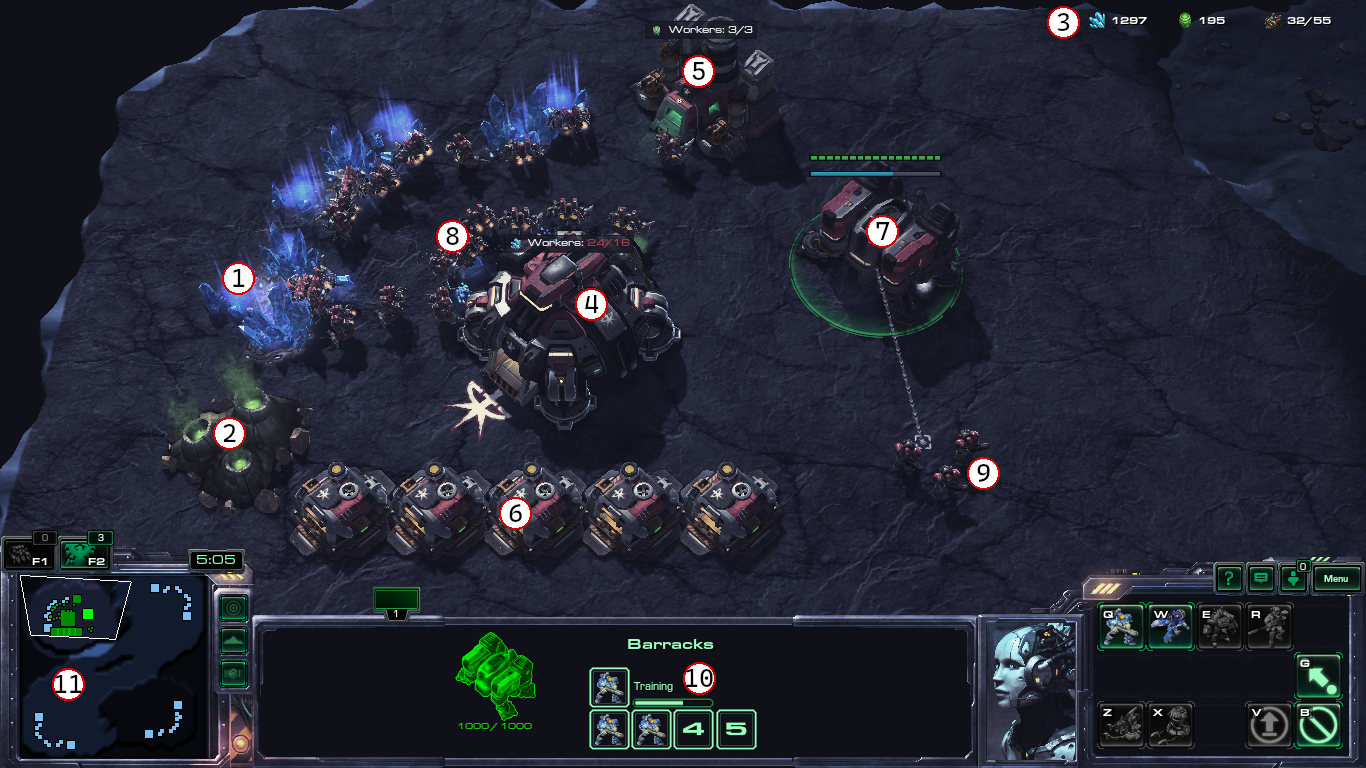
\includegraphics[width=1\textwidth]{figs/SC2_basic_elements.png}
    \caption[Basic elements of StarCraft II]{Basic elements of StarCraft II: (1) mineral deposits, (2) vespene gas geyser, (3) resource tracker (minerals, vespene, suppy), (4) Command Center, (5) Refinery, (6) Supply Depots, (7) Barracks, (8) SCVs (workers), (9) Marines (combat units), (10) unit queue, (11) minimap.}
    \label{fig:sc2_screenshot}
\end{figure}

\subsubsection{Resources}

There are three types of resources in StarCraft II: minerals, vespene gas and supply. Both minerals and vespene need to be collected from specific points in the map (mineral deposits and vespene geysers respectively) by sending worker units to collect the resource and bring it back to the closest town hall (the central structure of a base). In addition, to be able to collect vespene gas from a geyser, it is necessary to first build a specific structure on it (for example, the Terran's Refinery).

Minerals are used by all races to build and recruit most of their structures and units. Vespene gas is used in a similar way except that it is usually reserved for slightly more advanced structures and units.

Supply is different from the other two resources in several ways. First, it is not gathered from the map, but instead is earned by controlling certain structures or units, which vary depending on the race, and maxes out at 200. In the case of Terrans, for example, Command Centers provide 15 supply and Supply Depots provide 8. If any of the structures is destroyed, the supply will decrease accordingly. Second, unlike minerals and vespene, supply is not spent, simply allocated. Every unit type has a corresponding supply cost (usually 1 for basic units), and when a unit is created, it \say{occupies} that much supply, which is freed when the unit dies. Supply, then, limits how big a player's army can be.

\subsubsection{Structures and units}

Structures are stationary buildings from which units are created and upgrades are researched. The exact structures and their functions change from one race to another. All races have a main type of building referred to as a town hall (the Command Center for Terrans, for example) that serves as the central structure for a base by creating workers and receiving the minerals and vespene gas they harvest. In addition to the mineral and vespene cost that a structure might have, they also require a certain amount of time to build. Structures are not operable until their construction is finished.

As far as units go, they can be broadly placed in two categories: workers and combat units. Workers have the ability to build structures and gather resources while combat units are designed to damage enemy units and structures. Workers behave in a similar manner for all three races, whereas combat units are a lot more diverse. Similarly to structures, each unit type also takes a certain amount of time to train, on top of the mineral, vespene and supply cost. A single structure can only train one unit at a time, but up to five units can be queued (paying the mineral and vespene cost in advance) so that they begin training as soon as the previous one is completed.

In a typical game of StarCraft II, each player begins with one town hall and twelve workers placed next to several mineral deposits and two vespene geysers, as seen in figure \ref{fig:sc2_screenshot}.

\section{PySC2 library}

PySC2 is a python library developed by the Google Deep Mind team in collaboration with Blizzard \cite{Vinyals:2017}. It wraps the StarCraft II API and provides specifications for agent actions and environment observations, as well as a reward signal, which allow the use of the game as a reinforcement learning environment.

One of the major benefits of this library is that it can run the game tens of times faster than regular game-play. Internally, the game runs at 16 ticks per in-game second. When running the game at normal speed an in-game second matches a real-life second. PySC2 can run the game at much faster speeds, and we can configure how often (in terms of game ticks) it will stop the simulation, provide an observation and wait until our agent selects an action. For example, by setting the configuration value \texttt{step\_mul} to 32, PySC2 will poll our agent every 32 game ticks, which means the agent will act once every two in-game seconds.

\subsubsection*{Observation}

Every step, PySC2 supplies all the information about the current state of the game, both visually and through structured data. On the visual side, the agent has access to 27 feature layers, which are pixelated RGB representations of either the game screen or the mini-map (see figure \ref{fig:feature_layers}). Each feature layer displays different aspects of the game, such as the terrain height-map, the revealed parts of the map, units of a specific type or that belong to a specific player, etc. These layers are meant to allow agents to play the game using only (or mainly) visual information similar to that which a human player would have.

Additionally, the agents also have access to structured data about the state of the game, in the form of several tensors. These tensors contain numerical information about the players, resources and units in the map, as well as accumulated data such as total damage dealt or total resources spent.

\begin{figure}[h]
    \centering
    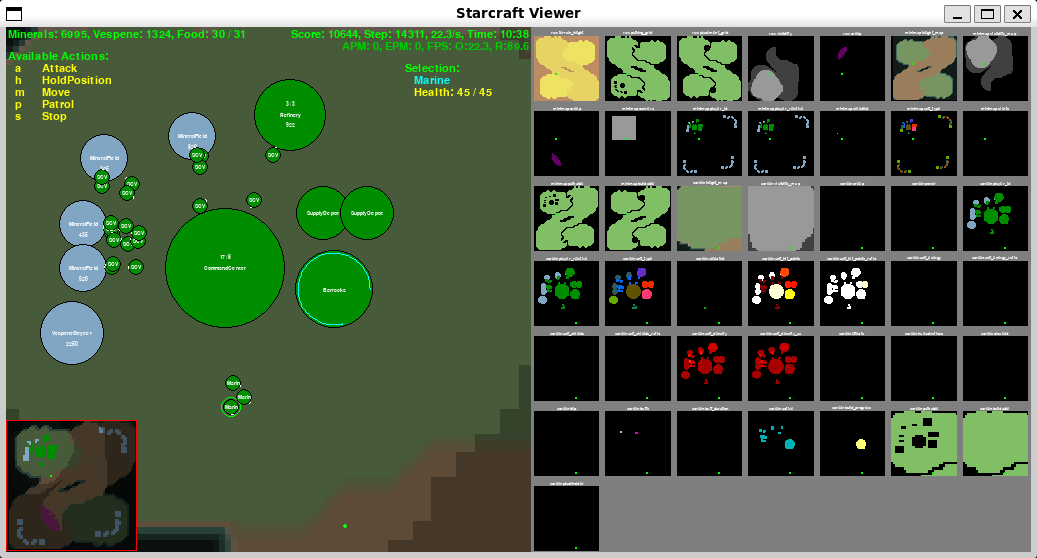
\includegraphics[width=1\textwidth]{figs/feature_layers.png}
    \caption{PySC2 feature layer view}
    \label{fig:feature_layers}
\end{figure}

\subsubsection*{Action space}

PySC2 allows the agents to interact with the game by calling functions that represent game actions that a regular player could take. These functions come in two forms. One type of function mimics the way a player would interact with the game, mostly by clicking the game area or the mini-map or pressing hot-keys. This includes clicking on the screen to select a unit, dragging a rectangle to select multiple units, clicking again to issue and order to move or attack, dragging the mouse to move the camera, etc.

The second type of function, called \say{raw function}, encodes higher level actions, such as attacking a specific point with one or more units, building a structure with a specific worker or sending a worker to gather resources. With these, the agent doesn't need to select units before giving the command, or move the camera to be able to see the area where it wants to build or attack. The library handles all the low level \say{basic} actions related to game-control that would combine to form a \say{raw function}.

\subsubsection*{Reward signal}

For each observation in a standard versus map, PySC2 provides two different rewards. One simply reflects the win or lose status at the end of a game: 1 for victory, -1 for defeat and 0 for draw (in case of a time-out). Every step during the game before the end of the match has a reward of 0. While this reward matches the desired behavior of the agents (we simply care about winning and not losing) it can be too sparse for the agents to properly learn, since the only receive one instance of reward after every game, which can easily take hundreds or thousands of steps.

For that reason, a second, dense reward is also included. This reward matches the internal score that the game assigns to each player. This score is calculated based on the amount of resources collected, upgrades researched, and unit and structures built. It is not a perfect metric to determine victory, but it serves as a decent estimator for which player is in a better position.

\subsection{Mini-games}

PySC2 comes with a selection of mini-games, created with the StarCraft II map editor, to serve as small environments with simpler objectives. These maps often have different reward signal to better match the goal of each mini-games.

\section{Simplified environment}

Since our goal is not to create an agent as proficient as possible in the game of StarCraft II and the scope of this project is relatively modest, we have decided to simplify the environment in a way that suits our needs.

\subsection{Race selection and technology progression}

Firstly, we have limited the race selection during all of our experiments to only one of the three races. That includes both our agents and the opponents they will fight against. The reason for this is that all three races are extremely different in many aspects of play. They create different units and structures, follow different progressions, interact with resources in different ways and are better suited for different strategies.

Similarly, we have also decided to have the agents work with only a fraction of the entire toolset available for the race. This is because the technology progression tree of structures, units and upgrades is far too expansive and nuanced for our scope.

Taking this into account, we have chosen the Terrans as the race to focus on since it can be considered the most simple and straight-forward of the three, and the one that functions best with a limited progression. The agents will have access to the following units and structures:

\begin{itemize}
    \item \textbf{Command Center:} Town hall for the Terran Race. It can recruit SCVs and is necessary to collect minerals and vespene. Every player begins the game with one Command Center next to a patch of mineral crystals. Costs 400 minerals and takes 71 seconds to build.
    \item \textbf{SCV:} Worker unit used to build all Terran structures and to collect minerals and vespene and take them to the closest Command Center. It has limited combat abilities, but we won't make use of them for the sake of simplicity. Every player begins the game with twelve SCVs. Costs 50 minerals and 1 supply, and takes 12 seconds to train.
    \item \textbf{Supply Depot:} Structure that increases the maximum supply of the player, which determines the amount of units the player can have at the same time. At least one Supply Depot is required to build a Barracks. Costs 100 minerals and takes 21 seconds to build.
    \item \textbf{Barracks:} Structure used to recruit new Marines. Costs 150 minerals and takes 46 seconds to build.
    \item \textbf{Marine:} Ranged combat unit capable of attacking and destroying enemy units and structures. It cannot harvest resources or build structures. Costs 50 minerals and takes 25 seconds to train.
\end{itemize}

Since we selected only the most basic units and structures, none of them require vespene gas, which means the agents will only need to work with minerals.

These units, although limited for a normal game of StarCraft II, are enough for the agents to perform the basic, general steps required to win the game. The expected strategy would be:

\begin{enumerate}
    \item Gather minerals with the starting SCVs and build new SCVs to speed up the process.
    \item Optionally, build a new Command Center near another source of minerals and more workers to improve the resource economy.
    \item Build a Supply Depot.
    \item Build a Barracks.
    \item Start recruiting Marines while continuing to build Supply Depots (to allow for more Marines) and Barracks (to recruit Marines faster).
    \item Attack the enemy base with the Marines.
\end{enumerate}

\subsection{Action space}
\label{sec:action_space}

To limit the action space to a more manageable level and to align with the limited progression described previously, we have decided on the following list of action for the agents:

\begin{itemize}
    \item \textbf{\texttt{NO\_OP:}} No action is taken for the current step.
    \item \textbf{\texttt{HARVEST\_MINERALS:}} Order a random idle worker to gather minerals from the closes mineral deposit.
    \item \textbf{\texttt{BUILD\_COMMAND\_CENTER:}} Order a random idle or harvesting worker to build a Command Center. The agent can only have up to three Command Centers.
    \item \textbf{\texttt{RECRUIT\_SCV\_0:}} Recruit an SCV on the first Command Center.
    \item \textbf{\texttt{RECRUIT\_SCV\_1:}} Recruit an SCV on the second Command Center.
    \item \textbf{\texttt{RECRUIT\_SCV\_2:}} Recruit an SCV on the third Command Center.
    \item \textbf{\texttt{BUILD\_SUPPLY\_DEPOT:}} Order a random idle or harvesting worker to build a Supply Depot. The agent can only have up to 24 Supply Depots.
    \item \textbf{\texttt{BUILD\_BARRACKS:}} Order a random idle or harvesting worker to build a Barracks. The agent can only have up to four Barracks.
    \item \textbf{\texttt{RECRUIT\_MARINE:}} Recruit a Marine on the Barracks with the shortest queue.
    \item \textbf{\texttt{ATTACK\_CLOSEST\_BUILDING:}} Attack with all Marines to the enemy building that is closest to the average position of all Marines.
    \item \textbf{\texttt{ATTACK\_CLOSEST\_WORKER:}} Attack with all Marines to the enemy worker that is closest to the average position of all Marines.
    \item \textbf{\texttt{ATTACK\_CLOSEST\_ARMY:}} Attack with all Marines to the enemy combat unit that is closest to the average position of all Marines.
    \item \textbf{\texttt{ATTACK\_BUILDINGS:}} Attack with all Marines to the enemy building that is closest to the average position of all enemy buildings.
    \item \textbf{\texttt{ATTACK\_WORKERS:}} Attack with all Marines to the enemy worker that is closest to the average position of all enemy workers.
    \item \textbf{\texttt{ATTACK\_ARMY:}} Attack with all Marines to the enemy combat unit that is closest to the average position of all enemy combat units.
\end{itemize}

For all building types, we have predefined all the position where they can be built for each map. The versus map we will use only supports up to two additional bases, which is why we limit the Command Centers to three (including the one each player starts with). The Supply Depots are limited to 24 since that is the amount that will bring the supply resource to its maximum of 200. Any Supply Depot beyond the 24\textsuperscript{th} will have no effect. The limit of four Barracks is somewhat arbitrary. Four is enough to build Marines at a sufficient speed to win the game.

When it comes to recruiting new units, we have allowed the agent to choose in which of its Command Centers to build the SCVs. Because assigning too many workers to harvest on the same mineral patch has diminishing returns, and since the harvest order always points the selected worker to the closest mineral deposit, this give the agent a certain amount of control on which of the bases' resource economy to develop.

As for the Marines, all Barracks are built next to the main base and close to each other, so there is no point in differentiating between them.

\subsection{Observation}

Even though the structured observation provided by PySC2 has a predictable form, it is variable enough that it cannot be used as-is as the input for a neural network. For that reason, and for the fact that it contains considerably more information than our agent could possible need, we have created our own observation data structure to represent the state of the game. Our observation contains mostly data obtained from PySC2's observation, plus some additional data that we calculate. The complete list of fields and their description can be found in appendix \ref{app:observation}, but some highlights include:

\begin{itemize}
    \item The amount of minerals the agent has.
    \item The number of each building type the agent has.
    \item The number of workers and Marines the agent has.
    \item The number of workers that are idle, building or harvesting and each Command Center.
    \item The distance from the Marines to various targets.
    \item The list of actions the agent can successfully take on the current step.
    \item The enemy's total army health.
\end{itemize}

We make no use of the visual information provided by the feature layers. This is because processing images would require the use of convolutional neural networks, which would be beyond our scope of complexity. Additionally, we have no need to make the agents play in the same way as humans, since that is not part of our goals.

\subsection{Reward signal}

The reward signals we have chosen will vary depending on the map and its objective. They are explained in detail in section \ref{sec:mini-games}.

\section{Custom scenarios}
\label{sec:mini-games}

We found that the mini-games distributed with PySC2 didn't fit with the needs and limitations of our different agents, which are explained in chapter \ref{chapter:implementation}. For that reason, we have used the StarCraft II map editor to create our own custom maps.

\subsubsection*{\texttt{BuildMarinesRandom}}

The objective of this mini-game is to recruit as many Marines as possible in a limited time-frame. The agent start with one Command Center and 16 SCVs next to a mineral patch. Additionally, to favour the exploration process, the scenario can randomly start with one Supply Depot already built, or one Supply Depot and one to four Barracks already built. The more advanced the starting base, the less likely it is.

The map has a fixed duration of 10 minutes. The score for each step is the amount of minerals spent on recruiting Marines since the last step. The agent has to build Supply Depots, Barracks and Marines in the most optimal way possible to maximize the score.

$$
r(t) = \texttt{spending\_Marines}_{t} - \texttt{spending\_Marines}_{t-1}
$$

\subsubsection*{\texttt{BuildMarinesFixed}}

This map is identical to \texttt{BuildMarinesRandom} except that it always start with only the Command Center and the SVCs. It is used for inference purposes.

\subsubsection*{\texttt{CollectMineralsRandom}}

The objective of this mini-game is to harvest as many minerals as possible in a limited time-frame. The agent start with one Command Center and 16 SCVs next to a mineral patch. The map includes two additional mineral patches to allow for up to two more bases to be built. Additionally, to favour the exploration process, the scenario can randomly start with one or two extra Command Centers already built. The more starting Command Centers, the less likely it is.

The map has a fixed duration of 12 minutes. The score for each step is the amount of minerals gained or lost since the last step. The agent has to build SCVs, Supply Depots, and Command Centers in the most optimal way possible to maximize the score.

$$
r(t) = \texttt{minerals}_{t} - \texttt{minerals}_{t-1}
$$

\subsubsection*{\texttt{CollectMineralsFixed}}

This map is identical to \texttt{CollectMineralsRandom} except that it always start with only one Command Center and the SVCs. It is used for inference purposes.

\subsubsection*{\texttt{DefeatBases}}

The objective of this mini-game is to defeat two small enemy bases. The agent starts with a group of Marines of variable size placed a random point close to the center of the map. The enemy bases consist of three Supply Depots, a small random number of SCVs and a small random number of Marines, randomly positioned on opposite corners of the map. The enemy Marines are programmed to attack any units that damage nearby buildings and the SCVs are programmed to repair nearby buildings. The number of ally and enemy Marines is set up so that the allies can destroy both bases reliably if played correctly.

The map ends when all enemy buildings have been destroyed or after 3 minutes. The score for each step is the change in health score since the last step, with an additional flat penalty each step to encourage faster episodes. The agent has to prioritize targeting enemy Marines, then SCVs and then buildings, and to focus on a single base at a time to maximize the score.

$$
\texttt{health\_score} = \texttt{health\_allies} \cdot 1.1 - \texttt{health\_enemies}
$$
$$
r(t) = \texttt{health\_score}_{t} - \texttt{health\_score}_{t-1} - \texttt{step\_cost}
$$

\subsubsection*{\texttt{Simple64}}

This is the only custom map included in PySC2 that we used without any changes. It is a two-player map, classified as a \say{melee} map instead of a mini-game, meaning the objective is simply to defeat the enemy player. Each player starts, randomly, in one of two opposite corners of a symmetric battlefield with a Command Center and 12 SCVs next to a mineral patch. This emulates a real game of StarCraft II.

The game ends when one of the player has been defeated (by losing all of their structures). It can also end in a draw if enough time passes with none of the players being able to gather more resources, produce more units or destroy enemy units. The score for each step is the change in a custom player score since the last step. The player score is calculated with the mineral value of all units of that player factored by the health or build progress of the unit.

$$
r(t) = (\texttt{ally\_score}_{t} - \texttt{enemy\_score}_{t}) - (\texttt{ally\_score}_{t-1} - \texttt{enemy\_score}_{t-1})
$$
\chapter{Experiments}
\label{chapter:experiments}

In this chapter we discuss the implementation details of the project, the training process for the agents and the results we have obtained.

\section{Implementation}

As was mentioned in chapter \ref{chapter:introduction}, this project is a continuation of previous works by other students. As such, we have decided to use the existing codebase as a starting point. The entire code, as well as the custom mini-games and trained models, is available in our public GitHub repository\footnote{\url{https://github.com/DavidPerezGomez/tfm-rl-starcraft2}}.

\subsection{Agent structure}
\label{sec:agent_structure}

Our agents implement the Deep Q-Learning algorithm described in section \ref{sec:dql}. They include two neural networks (main and target) to learn to estimate the value of state-action pairs, and a replay buffer to store previous experiences as training samples for the networks. They also implement the $\epsilon$-greedy method to favour exploration during the entire training process.

\subsubsection*{Networks}

The neural networks, including optimizer and scheduler, are implemented using PyTorch. They are fully connected multilayer perceptrons. Since the size and shape of neural networks can have a large impact on their performance and ability to learn, we have defined three increasingly complex configurations for the hidden layers to use throughout the project:

\begin{itemize}
    \item \textbf{Medium:} Has four hidden layers with 128, 128, 64 and 32 neurons respectively.
    \item \textbf{Large:} Has five hidden layers with 256, 128, 128, 64 and 32 neurons respectively.
    \item \textbf{Extra large:} Has size hidden layers with 512, 256, 128, 128, 64 and 32 neurons respectively.
\end{itemize}

\subsubsection*{Action implementation}

To implement the actions described in section \ref{sec:action_space} we use the following raw actions from the PySC2 API:

\begin{itemize}
    \item \textbf{\texttt{Harvest\_Gather\_unit}:} Given a worker unit and a mineral patch, it commands the worker to harvest minerals from the patch.
    \item \textbf{\texttt{Train\_SCV\_quick}:} Given a Command Center, it begins training an SCV in the Command Center.
    \item \textbf{\texttt{Build\_CommandCenter\_pt}:} Given an SCV and a coordinates point in the map, it commands the SCV to build a Command Center on the specified position.
    \item \textbf{\texttt{Build\_SupplyDepot\_pt}:} Given an SCV and a coordinates point in the map, it commands the SCV to build a Supply Depot on the specified position.
    \item \textbf{\texttt{Build\_Barracks\_pt}:} Given an SCV and a coordinates point in the map, it commands the SCV to build a Barracks on the specified position.
    \item \textbf{\texttt{Train\_Marine\_quick}:} Given a Barracks, it begins training a Marine in the Barracks.
    \item \textbf{\texttt{Attack\_unit}:} Given two units, it commands the first one to move and attack towards the second one.
\end{itemize}

\subsubsection*{Action masking}

\begin{figure}[t]
    \begin{equation*}
        \begin{bmatrix}
        q_1 \\ q_2 \\ q_3 \\ q_4 \\ \vdots \\ q_n
        \end{bmatrix}
        \times 
        \begin{bmatrix}
        1 \\ 0 \\ 0 \\ 1 \\ \vdots \\ 0
        \end{bmatrix}
        \Rightarrow 
        \begin{bmatrix}
        q_1 \\ -\infty \\ -\infty \\ q_4 \\ \vdots \\ -\infty
        \end{bmatrix}
    \end{equation*}
\caption{Application of action masking}
\label{fig:action_masking}
\end{figure}

Action masking is a technique used to prevent a reinforcement learning agent from selecting actions that would be invalid for the current state, such as training a Marine without enough resources or an available Barracks, for example. It has been shown to improve learning efficiency in complex action spaces \cite{Huang:2022}. The previous work implemented action masking during exploitation, but not during training. Instead, if an invalid action was selected, it would be transformed into a \texttt{NO\_OP} action, but the agent would still learn based on the action it originally selected.

For this project, we have decided to apply action masking during training as well. Part of the reason for this is that using action masking only during inference means that the agent will sometimes be prevented from following the policy that it has learned, which prevent us from accurately evaluating said policy. Another reason is that the conversion from invalid actions to \texttt{NO\_OP} during training can cause the agent to learn to use invalid actions as a proxy for the \texttt{NO\_OP} action. This would not be a desired behavior, since we want the agent to be deliberate when selecting actions.

To implement action masking, whenever an agent needs to select an action we use custom logic to determine which actions would be invalid for the current state and apply that mask to the q-values generated by the neural network, converting the values associated with the invalid actions into negative infinity (figure \ref{fig:action_masking}). The agent then selects the action with the highest q-value, which necessarily excludes the invalid actions. Since the \texttt{NO\_OP} is always valid, the agents will always have at least one valid action available.

It should be noted that whenever we make use of random agents (be it as baselines to compare the performance of RL agents or as opponents in versus maps), we also apply action masking, allowing them to select randomly only from the set of valid actions.

\subsubsection*{Action frequency}

In section \ref{sec:pysc2} we explained how PySC2 allows us to configure how often the agent will be able to act on the environment. Setting the action frequency too low can obviously lead to poor performance, since the agent would be too slow to react to events taking place in the game. Setting it too high, however, can present its own set of challenges. For one, it amplifies the sparse and long-term reward issues present in the environment: the more observations and actions the agent takes, the more \say{perceived} time it will take for long-term investments to pay off. Second, StarCraft II is a relatively slow paced game, where situations don't change drastically in an instant. Two observations taken in a very short time will be almost identical in most situations, slowing down the training process.

In the end, we have settled on acting every 32 game ticks (2 in-game seconds), which we think strikes a decent balance.

\subsubsection*{Custom scenarios}

Lastly, we found that the mini-games distributed with PySC2 didn't fit with the needs and limitations of our different agents. For that reason, we have used the StarCraft II map editor to create our own custom maps. These are described in section \ref{sec:training} alongside each of the agents that were trained in them.

\subsection{Hierarchical model}

\begin{figure}[t]
    \centering
    \begin{subfigure}[b]{0.45\textwidth}
        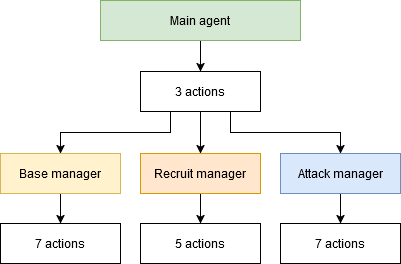
\includegraphics[width=1\textwidth]{figs/multi_agent_schema.png}
        \caption{Hierarchical agent schema}
        \label{fig:multi_schema}
    \end{subfigure}
    \hspace{1cm}
    \begin{subfigure}[b]{0.25\textwidth}
        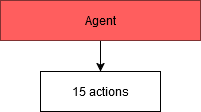
\includegraphics[width=1\textwidth]{figs/single_agent_schema.png}
        \caption{Single agent schema}
        \label{fig:single_schema}
    \end{subfigure}
    \hfill
    \caption{Agents' structure}
\end{figure}

Our Hierarchical model consists of four different agents: one high-level manager and three lower-level sub-agents, as depicted in figure \ref{fig:multi_schema}. The main agent, also called game manager, is tasked with selecting which of the sub-agents will decide the next several actions. For that purpose, instead of the set of actions described in section \ref{sec:action_space}, it works with a different, exclusive list of actions:

\begin{itemize}
    \item \textbf{\texttt{EXPAND\_BASE}:} Delegate the action selection to the base manager sub-agent.
    \item \textbf{\texttt{EXPAND\_ARMY}:} Delegate the action selection to the recruit manager sub-agent.
    \item \textbf{\texttt{ATTACK}:} Delegate the action selection to the attack manager sub-agent.
\end{itemize}

Action masking is not applied to these action.

The main agent will also implement a temporal extension of five steps, meaning that it will act only every five steps (160 game ticks, 10 in-game seconds), as explained in \ref{sec:hrl}.

\subsubsection*{Attack manager sub-agent}

The attack manager sub-agent is in charge of using the Marine army to destroy the enemy units and structures. It has access to the following actions:

\begin{multicols}{2}
\begin{itemize}
    \item \textbf{\texttt{NO\_OP}}
    \item \textbf{\texttt{ATTACK\_CLOSEST\_BUILDING}}
    \item \textbf{\texttt{ATTACK\_CLOSEST\_WORKER}}
    \item \textbf{\texttt{ATTACK\_CLOSEST\_ARMY}}
    \item \textbf{\texttt{ATTACK\_BUILDINGS}}
    \item \textbf{\texttt{ATTACK\_WORKERS}}
    \item \textbf{\texttt{ATTACK\_ARMY}}
\end{itemize}
\end{multicols}

It can choose what type of enemy unit to attacks and whether to target whichever is closest or the biggest cluster of enemies. Although it has access to the \texttt{NO\_OP} action, it will be prevented from selecting it, through action masking, unless every other action is unavailable (in the case that the agent has no marines or there are no enemy units). This is because the game has an automatic targeting system where an idle combat unit that is in range of enemy units will start attacking them while prioritizing targets according to the game's AI. Using this, the agent could learn a \say{launch and forget} strategy by sending the marines to attack the enemy and then simply waiting and letting the game's AI control most of the fight. Since our goal is to keep the environment and action space more complex than the previous work, we want the agent to be forced to take a more active role.

\subsubsection*{Recruit manager sub-agent}

The recruit manager sub-agent is in charge of training the Marine army by creating Barracks and recruiting Marines. It has access to the following actions:

\begin{multicols}{2}
\begin{itemize}
    \item \textbf{\texttt{NO\_OP}}
    \item \textbf{\texttt{HARVEST\_MINERALS}}
    \item \textbf{\texttt{BUILD\_SUPPLY\_DEPOT}}
    \item \textbf{\texttt{BUILD\_BARRACKS}}
    \item \textbf{\texttt{RECRUIT\_MARINE}}
\end{itemize}
\end{multicols}

Since performing an action to build structures while there are no idle workers will cause a harvesting worker to stop gathering minerals, the agent has the ability to send workers back to harvesting, so as to not cripple the resource economy by accident, specially when working by itself during training.

\subsubsection*{Base manager sub-agent}

The base manager sub-agent is in charge of developing the resource economy by creating more workers and Command Centers. It has access to the following actions:

\begin{multicols}{2}
\begin{itemize}
    \item \textbf{\texttt{NO\_OP}}
    \item \textbf{\texttt{HARVEST\_MINERALS}}
    \item \textbf{\texttt{BUILD\_COMMAND\_CENTER}}
    \item \textbf{\texttt{RECRUIT\_SCV\_0}}
    \item \textbf{\texttt{RECRUIT\_SCV\_1}}
    \item \textbf{\texttt{RECRUIT\_SCV\_2}}
    \item \textbf{\texttt{BUILD\_SUPPLY\_DEPOT}}
\end{itemize}
\end{multicols}

It has the ability to build Supply Depots because the amount of workers is also limited by the supply resource. Although each Command Center provides some supply, it is not enough to reach the optimal worker amount, and some Supply Depots are necessary at some point.

\section{Training}
\label{sec:training}

Training the RL agents proved to be more challenging than expected. We have gone through many revision of the training mini-games and reward signals for each for the sub-agents, main hierarchical agent and single agent. In general, the agents had trouble converging, often finding a good solution part way through the training, only to then collapse and spiral toward considerably worse policies as the training continued. We had to make use of frequent checkpoints to get versions of the agents with effective policies. The increasing values for the training loss that can be seen in appendix \ref{app:stats} suggest that the frequency at which we synchronize the target network with the main network may be too high, but we were unable to test more configurations due to time limitations.

\begin{figure}[t]
    \centering
    \begin{subfigure}[b]{0.45\textwidth}
        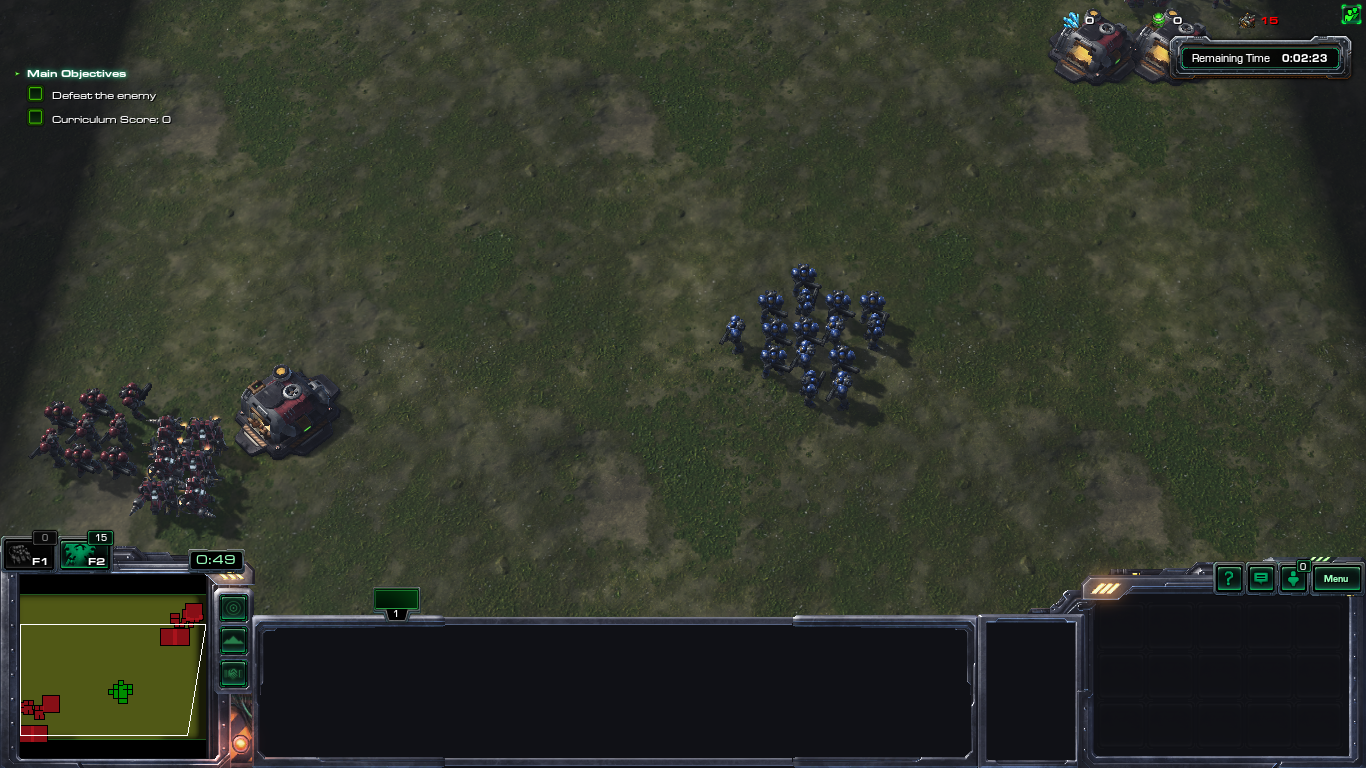
\includegraphics[width=1\textwidth]{figs/DefeatBases.png}
        \caption{\texttt{DefeatBases} mini-game}
        \label{fig:DefeatBases}
    \end{subfigure}
    \hfill
    \begin{subfigure}[b]{0.45\textwidth}
        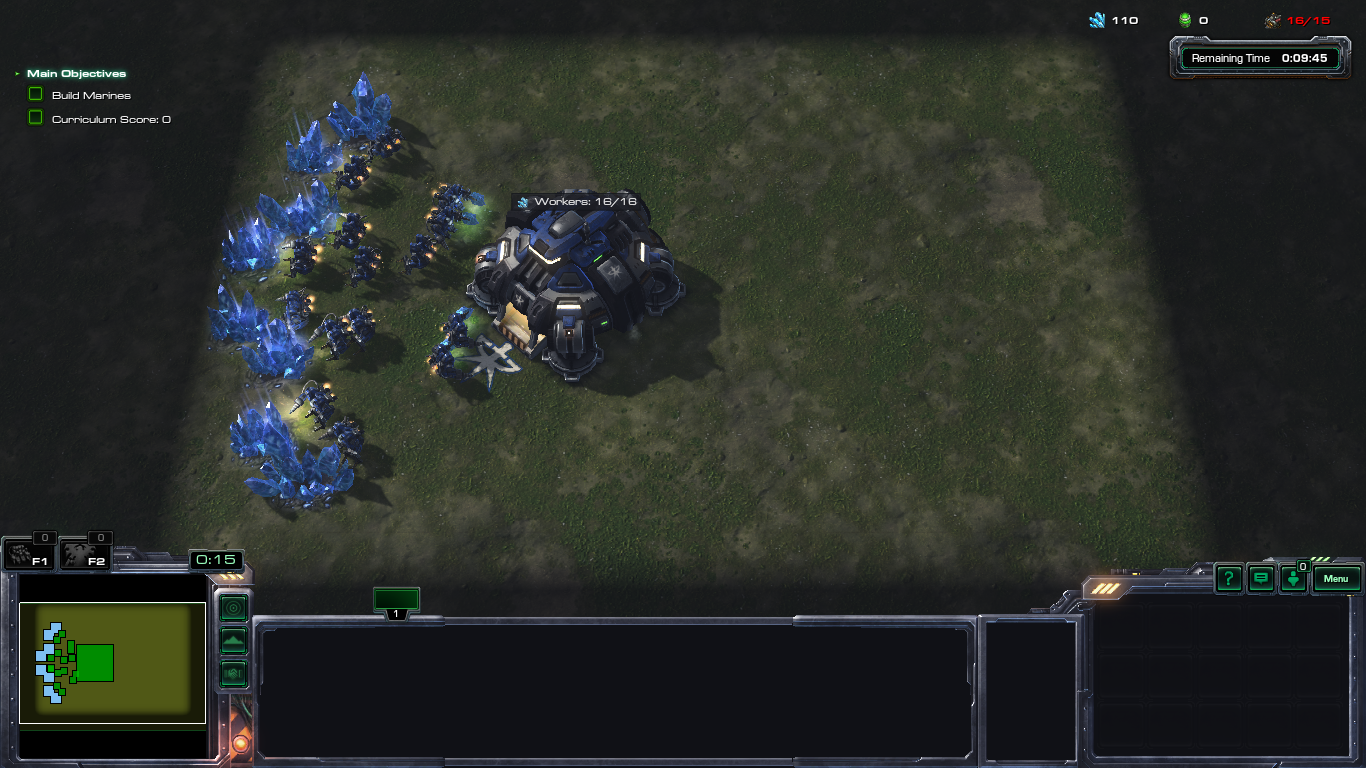
\includegraphics[width=1\textwidth]{figs/BuildMarinesFixed.png}
        \caption{\texttt{BuildMarinesFixed} mini-game}
        \label{fig:BuildMarinesFixed}
    \end{subfigure}
    \hfill
    \begin{subfigure}[b]{0.45\textwidth}
        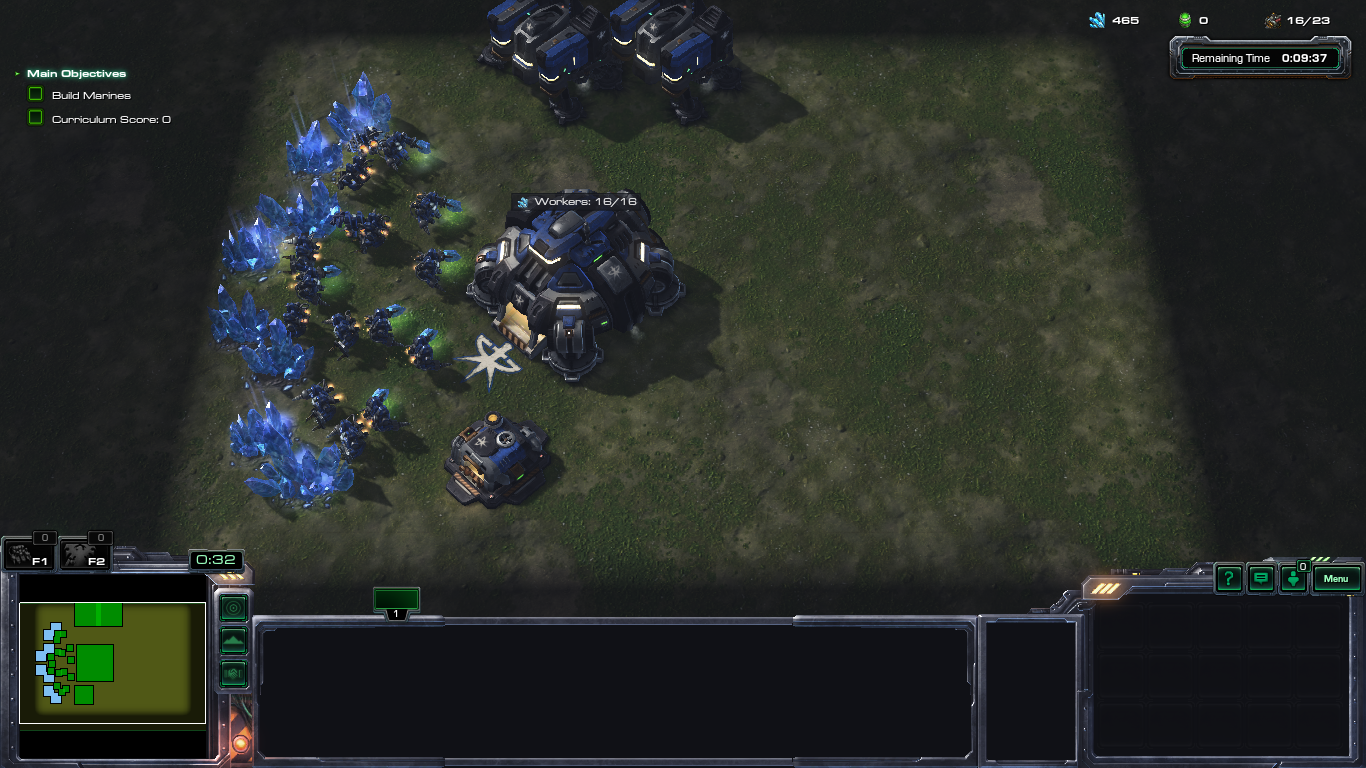
\includegraphics[width=1\textwidth]{figs/BuildMarinesRandom.png}
        \caption{\texttt{BuildMarinesRandom} mini-game}
        \label{fig:BuildMarinesRandom}
    \end{subfigure}
    \hfill
    \begin{subfigure}[b]{0.45\textwidth}
        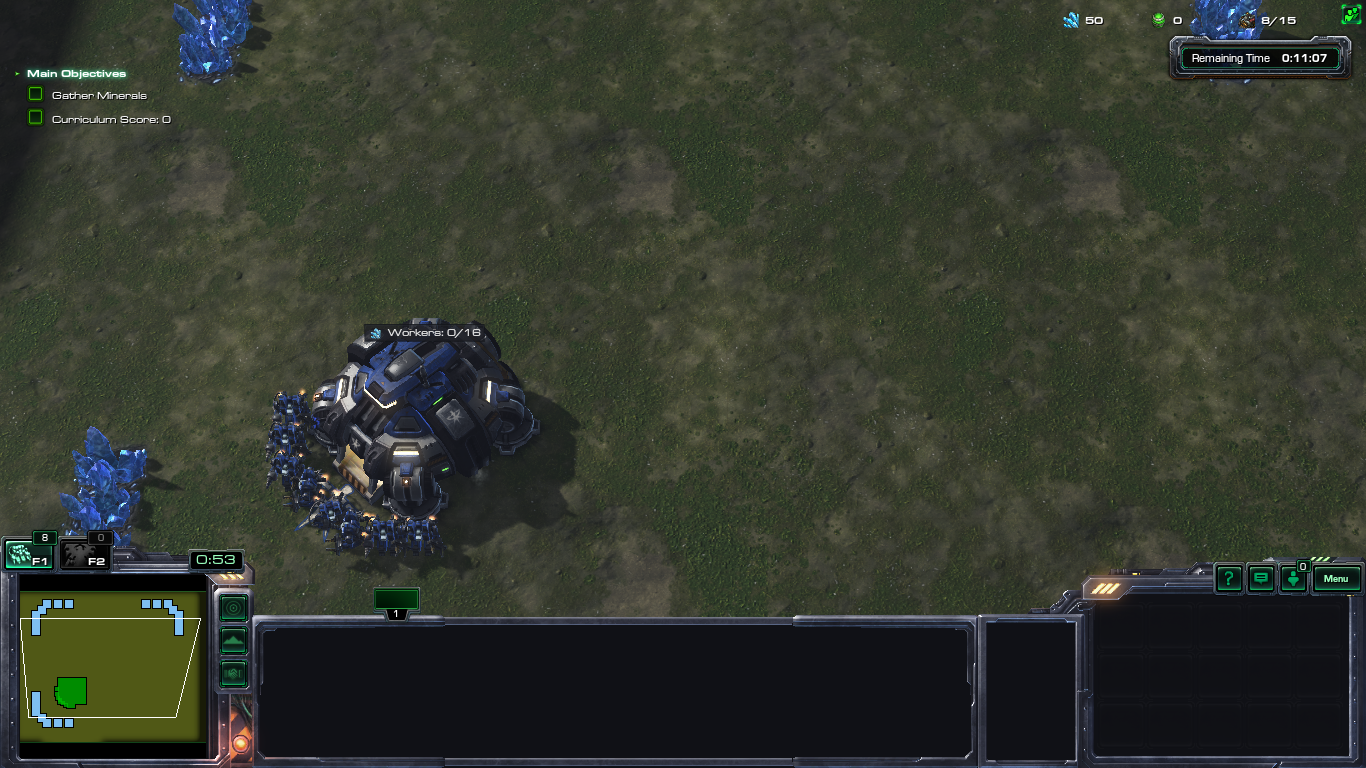
\includegraphics[width=1\textwidth]{figs/SaturateHarvesters.png}
        \caption{\texttt{SaturateHarvesters} mini-game}
        \label{fig:SaturateHarvesters}
    \end{subfigure}
    \caption{Custom mini-games}
\end{figure}

\subsection{Attack manager}

The pre-existing PySC2 mini-games that center around combat focus only on enemy combat units, and none include workers or structures, which we want so that the agent gets more complete observations and learns the new attack actions with specific targets. Additionally, the enemy units used are always from the Zerg race, which doesn't represent the type of opposition that the agent will find in the final versus map. For those reasons, we have created a new mini-game called \texttt{DefeatBases} (figure \ref{fig:DefeatBases}).

The objective of this mini-game is to destroy two small enemy bases. The agent starts with a group of Marines of variable size placed a random point close to the center of the map. The enemy bases consist of three Supply Depots, a small random number of SCVs and a small random number of Marines, randomly positioned on opposite corners of the map. The enemy Marines are programmed to attack any units that damage nearby buildings and the SCVs are programmed to repair nearby buildings. The number of ally and enemy Marines is set up so that the allies can destroy both bases reliably if played correctly. The map ends when all enemy buildings have been destroyed or after 3 minutes.

For this agent, we have created a reward signal that encourages destroying the enemy units and structures quickly while losing as few of the agent's own marines as possible. The score calculated for each step is the difference in health of all ally units and all enemy units. The reward for the agent is the change in score from the previous step, with an additional flat penalty to encourage faster episodes. The agent has to prioritize targeting enemy Marines, then SCVs and then buildings, and to focus on a single base at a time to maximize the reward.

$$
r(t) = \Delta(\texttt{health\_allies}_{t} - \texttt{health\_enemies}_{t}) - \texttt{step\_cost}
$$

The sub-agent uses a medium neural network and has been trained for 6147 steps (150 episodes). Figure \ref{fig:DefeatBases_scores} shows the scores obtained by the trained agent during exploitation compared to the ones obtained by a random agent.

\begin{figure}[t]
    \centering
    \begin{subfigure}[b]{0.48\textwidth}
        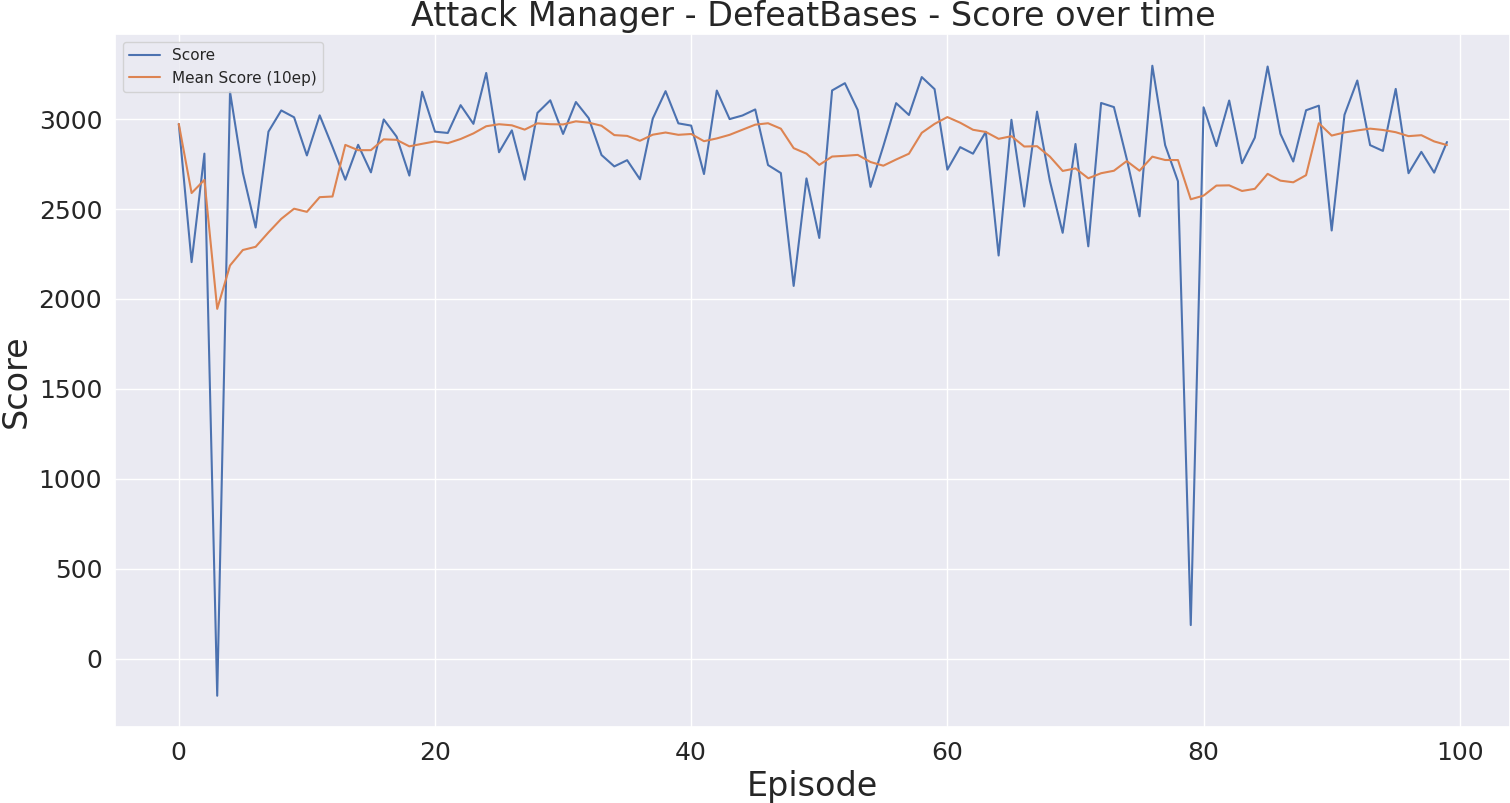
\includegraphics[width=1\textwidth]{figs/multi_dqn_army_attack_manager/exploit/score.png}
        \caption{Attack manager sub-agent score}
    \end{subfigure}
    \hfill
    \begin{subfigure}[b]{0.48\textwidth}
        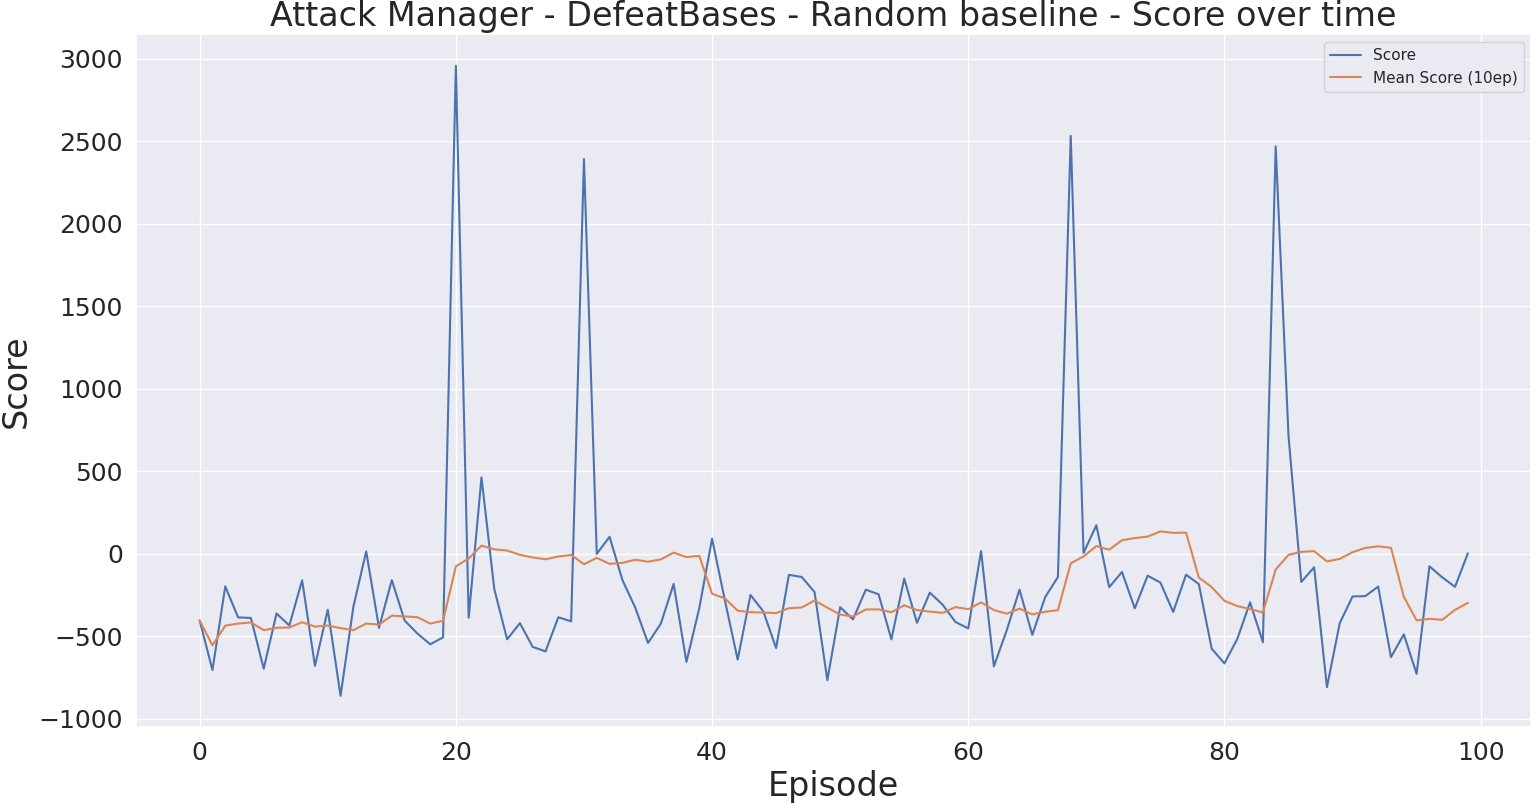
\includegraphics[width=1\textwidth]{figs/multi_random_army_attack_manager/exploit/score.png}
        \caption{Random baseline score}
    \end{subfigure}
    \caption{Scores for \texttt{DefeatBases} mini-game}
    \label{fig:DefeatBases_scores}
\end{figure}

\subsection{Recruit manager}

For this sub-agent we have created a mini-game called \texttt{BuildMarinesFixed} (figure \ref{fig:BuildMarinesFixed}) based on the existing \texttt{BuildMarines} PySC2 mini-game, with a few tweaks to the score handling to adjust it to our training pipeline but keeping the parameters and gameplay of the original unchanged.

The objective of this mini-game is to recruit as many Marines as possible in a limited time frame. The agent starts with one Command Center and 16 SCVs next to a mineral patch, and the map ends after 10 minutes. The agent has to build Supply Depots, Barracks and Marines in the most optimal way possible to maximize the reward.

The first reward signal we decided for this agent was simply a flat reward every time a Marine completed training. This reward has the peculiarity that it is always delayed in time. Since a Marine takes 25 seconds to train, the reward for taking the \texttt{RECRUIT\_MARINE} action will always be received 13 steps later. This shouldn't be a big problem since Q-Learning is capable of handling delayed rewards; and, indeed, the agent was able to learn an effective strategy. However, for reasons explained later in section \ref{sec:hierarchical_agent}, we decided to make the reward signals as instantaneous as possible.

The score for the recruit manager sub-agent is the amount of minerals spent on training marines, and the reward for each step is the change in score. Because the minerals are spent as soon as a Marine begins training and not when it ends, the reward is received immediately. There is no flat penalty every step because the mini-game has a fixed duration so it is not possible to make it end faster

$$
r(t) = \Delta(\texttt{marines\_spending}_{t})
$$

We also experimented penalizing the agent for spending minerals on anything other than Marines, even Supply Depots and Barracks which are necessary to begin training Marines. Our hope was that that would lead to more optimal and less wasteful strategies. While that may still be true, that reward signal caused even more instability during training and exacerbate the convergence difficulties mentioned previously. For that reason, and time limitations, we simplified the reward to the one described above.

While training this sub-agent we noticed that the exploration process was constantly falling into the same patterns. Since Supply Depots are cheaper to build that Barracks and impossible actions are masked, it means that while the agent has enough minerals to build a Supply Depot but not enough to build a Barracks, the only actions it can take are either \texttt{NO\_OP}, or \texttt{BUILD\_SUPPLY\_DEPOT}. The random actions during exploration almost guarantee that the agent would build the Supply Depot before amassing enough minerals to build a Barracks, restarting the process, and only getting to build Barracks once no more Supply Depots could be built. While it wasn't impossible for the agent to randomly build a Barracks before all 24 available Supply Depots, it was infrequent, and building two, three or four Barracks, even more so.

Since the reward signal is never negative, it cannot \say{disuade} the agent from taking certain actions. Because of that, the agent relies heavily on exploration to discover which course of action provides a greater benefit. To favour the exploration process, we have created a second mini-game, \texttt{BuildMarinesRandom} (figure \ref{fig:BuildMarinesRandom}). This map is identical to \texttt{BuildMarinesFixed} except that the scenario can randomly start with one Supply Depot already built, or one Supply Depot and one to four Barracks already built. The more advanced the starting base, the less likely it is. Additionally, the amount of minerals that the agent has at the start of the episode is uniformly distributed from 50 to 500 in increments of 10. This way, we present the agent with different situations to explore.

The agent uses a medium neural network and has been trained for 9000 steps (30 episodes) on \texttt{BuildMarinesRandom} for an initial exploration phase, and then for 9000 steps (30 episodes) more in \texttt{BuildMarinesFixed}, to adapt its strategy to an environment more closely resembling the final versus map. When evaluating the performance of the agent, we use \texttt{BuildMarinesFixed} exclusively, for a standardized environment. Figure \ref{fig:BuildMarinesFixed_scores} shows the scores obtained by the trained agent during exploitation compared to the ones obtained by a random agent.

\begin{figure}[t]
    \centering
    \begin{subfigure}[b]{0.48\textwidth}
        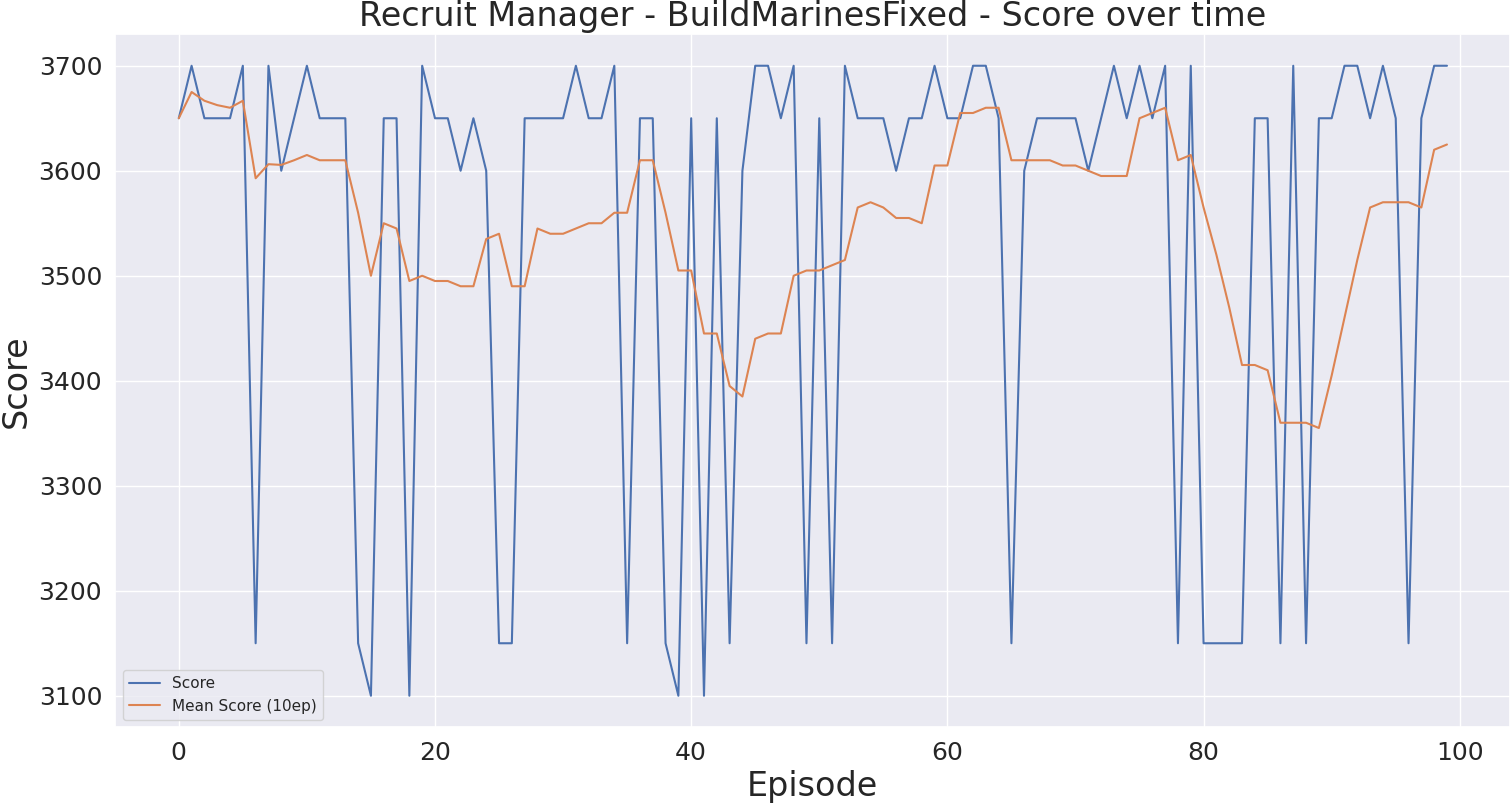
\includegraphics[width=1\textwidth]{figs/multi_dqn_army_recruit_manager/exploit/score.png}
        \caption{Recruit manager sub-agent score}
    \end{subfigure}
    \hfill
    \begin{subfigure}[b]{0.48\textwidth}
        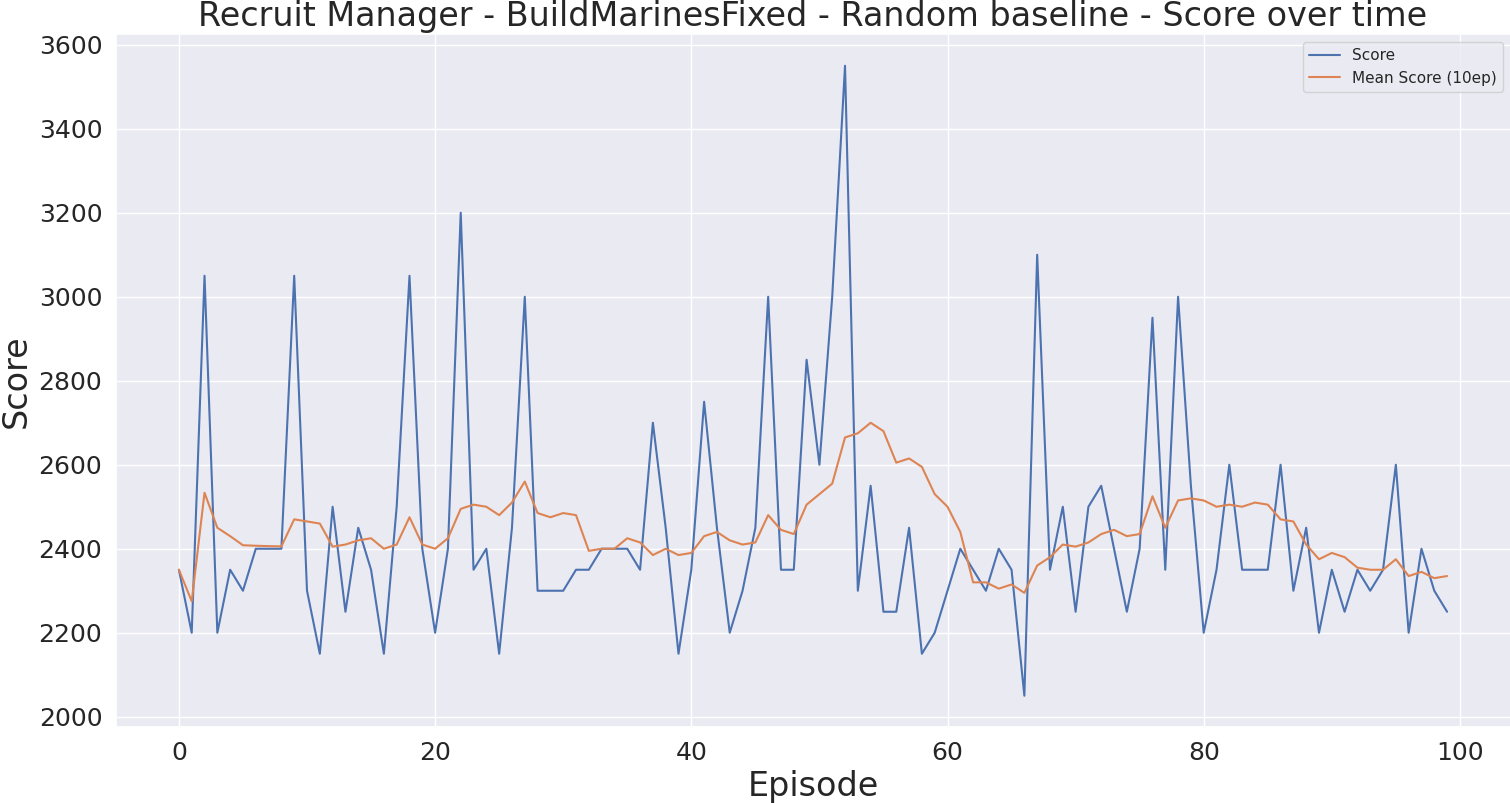
\includegraphics[width=1\textwidth]{figs/multi_random_army_recruit_manager/exploit/score.png}
        \caption{Random baseline score}
    \end{subfigure}
    \caption{Scores for \texttt{BuildMarinesFixed} mini-game}
    \label{fig:BuildMarinesFixed_scores}
\end{figure}

\subsection{Base manager}

One of the mini-games in the PySC2 suite centers around harvesting resources (both minerals and vespene gas) and it is close to what we need for this sub-agent. That map, however, only supports up two bases (two Command Centers) while, in the final versus map, the agent can have up to three. Because of that, we have create a new mini-game, \texttt{Saturate\_Harvesters} (figure \ref{fig:SaturateHarvesters}), expanding the existing one and removing the vespene geysers since our agent doesn't make use of them.

The objective of this mini-game is to harvest as many minerals as possible in a limited time frame. The agent starts with one Command Center and eight SCVs next to a mineral patch. The map includes two additional mineral patches to allow for up to two more bases to be built. The map has a fixed duration of 12 minutes.

We experimented with several different reward signals for this map such as the amount of minerals collected since last step, the net change in minerals since las step (which would penalize for spending minerals) and the change in mineral gathering rate (measured in minerals per second). However, all of these are long-term rewards: the benefit of training a new worker and assigning it to harvest minerals is gaining 5 additional minerals every so often for the remainder of the episode. As was the case with the recruit manager, Q-Learning can learn what states lead to better long-term rewards. But as mentioned previously, we favoured the use of immediate reward signals.

We have settled on calculating the score based on the efficiency of the harvesting workers. A Command Center can have any number of workers harvesting resources towards it. However, the optimum number of harvesters depends on the number of nearby mineral deposits. There has been extensive work studying the resource economy of StarCraft II\footnote{\url{https://liquipedia.net/starcraft2/Mining_Minerals}}, but to summarize, for every mineral deposit, the first two workers mining on it will operate at full efficiency, the third worker will operate at roughly half efficiency, and any workers past the third are completely redundant. Since both in the mini-game and in the final versus map each mineral patch contains eight mineral deposits, the maximum number of effective harvesters for each Command Center is 24, with the first 16 being the most valuable. Using that, we calculate the harvesting efficiency score by adding the amount of harvesters up to 16 plus half the amount of harvesters between 16 and 24 on each Command Center. The reward, then, is the change in score from the previous step minus a flat penalty. This way, the reward increases or decreases immediately when an worker is ordered to harvest or when a harvesting worker is ordered to do something else like build a structure. The penalty is removed if the maximum efficiency has been achieved since the agent can no longer improve the efficiency.

$$
r(t) = \Delta(\texttt{harvester\_efficiency}_{t}) - \texttt{step\_cost}
$$

The agent uses a medium neural network and has been trained for 18000 steps (50 episodes). Figure \ref{fig:SaturateHarvesters_scores} shows the scores obtained by the trained agent during exploitation compared to the ones obtained by a random agent.

\begin{figure}[t]
    \centering
    \begin{subfigure}[b]{0.48\textwidth}
        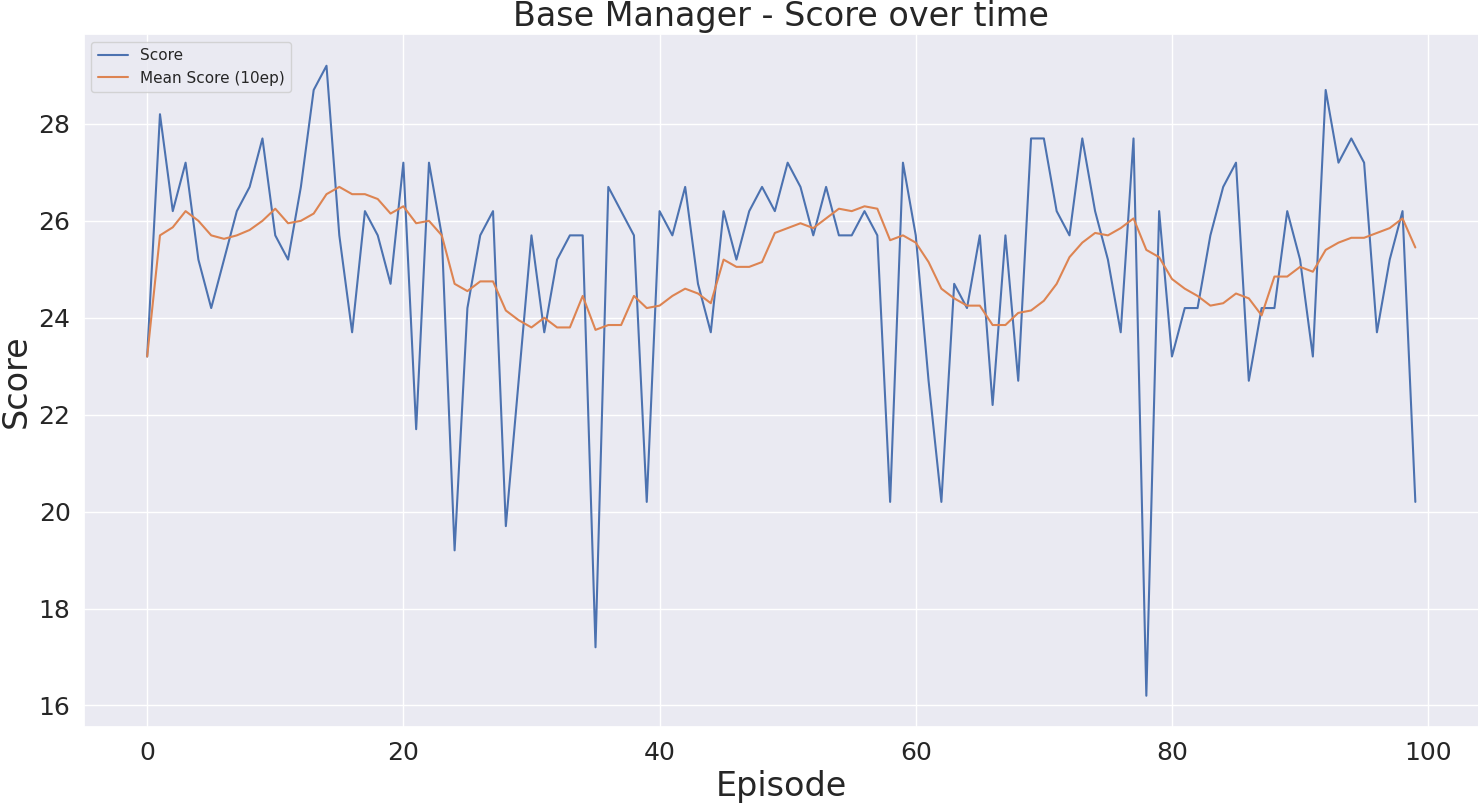
\includegraphics[width=1\textwidth]{figs/multi_dqn_base_manager/exploit/score.png}
        \caption{Base manager sub-agent score}
    \end{subfigure}
    \hfill
    \begin{subfigure}[b]{0.48\textwidth}
        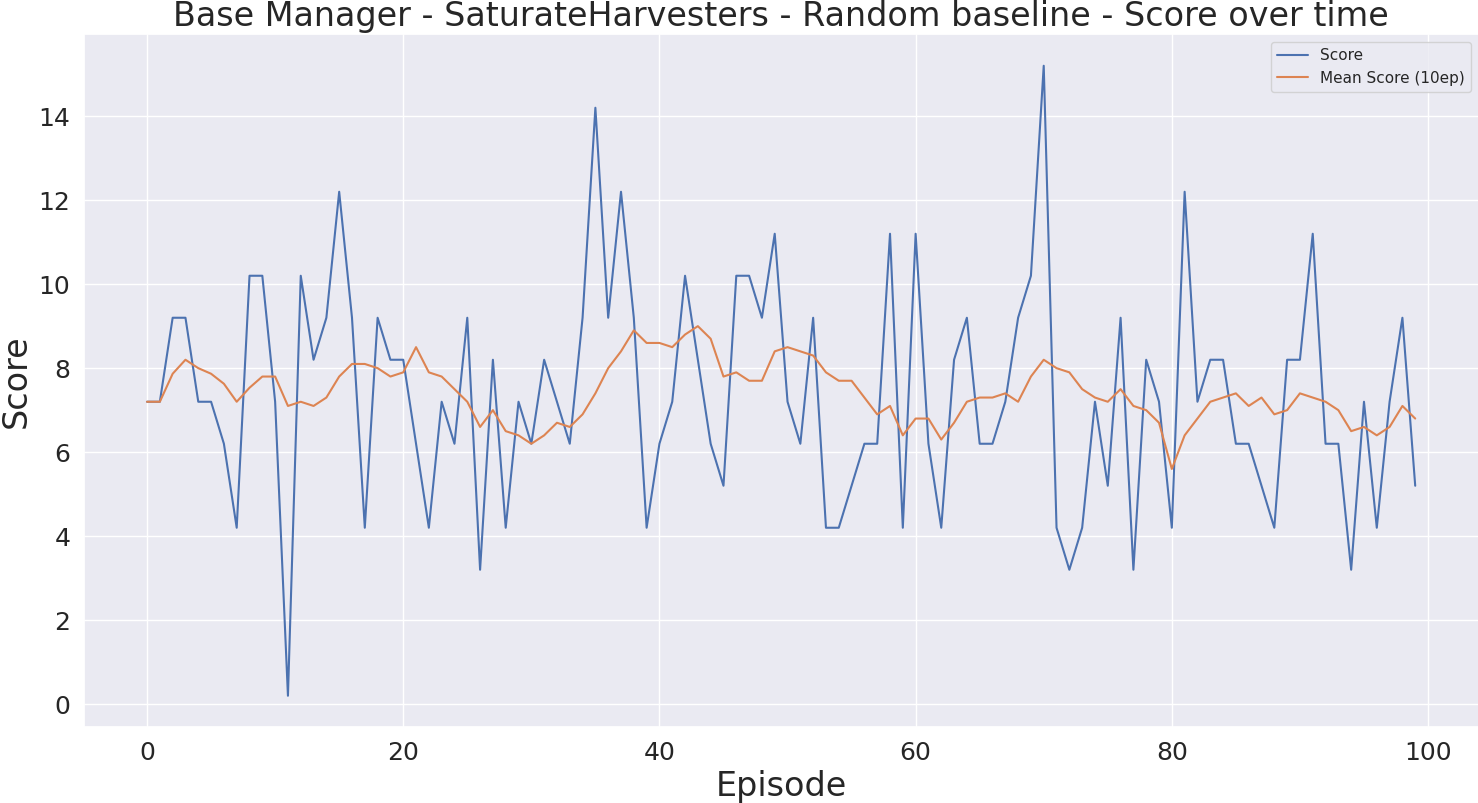
\includegraphics[width=1\textwidth]{figs/multi_random_base_manager/exploit/score.png}
        \caption{Random baseline score}
    \end{subfigure}
    \caption{Scores for \texttt{SaturateHarvesters} mini-game}
    \label{fig:SaturateHarvesters_scores}
\end{figure}

\subsection{Hierarchical agent}
\label{sec:hierarchical_agent}

To train the hierarchical agent we have used the existing PySC2 melee map \texttt{Simple\_64}. It a relatively small \say{Z}-shaped 1v1 versus map. Both players start on opposite corners of the map with a Command Center and 12 SCVs. The remaining two corners hold mineral patches to allow for additional bases. The goal of the map is simply to win the match by destroying all of the opponent's structures. The game can also end in a draw if enough time passes with none of the players being able to gather more resources, produce more units or destroy enemy units. When playing this map, both during training and evaluation, the opponent is controlled by a random agent.

As explained in \ref{sec:reward_signal} using a reward signal based on wins and losses can be problematic due to it being too sparse. We experimented with different ways to calculate the reward until we settled on the following: we calculate a value for both players based on the total mineral value of their units and structured factored by their health percentage (with a minimum factor of $0.5$ since even a badly damaged unit or structure is equally effective at its job). This value is capped at $4000$. The score for the agent, then, is the difference between its value and the opponent's, and the reward is the change in score from the previous step with an additional step penalty.

$$
r(t) = \Delta(\max(\texttt{agent\_score}_{t}, 4000) - \max(\texttt{enemy\_score}_{t}, 4000)) - \texttt{step\_cost}
$$

The agent also receives an additional large reward or penalty on the last step of each episode according to the result of the game: $5000$ in case of a victory, $-5000$ in case of defeat and $0$ in case of a draw.

The reason for the maximum score is to disincentivize stalling when a the game is almost over. Without it, the agent could easily get in a position where the enemy is no longer a threat and then keep growing its army at a rate where the reward is greater than the step cost, not only wasting time, but also risking a draw after enough time. This way, past a certain point, the only way to continue getting rewards is to cause damage to the opponent.

The training of the hierarchical agent is divided in two steps: fine-tuning of the sub-agents and training of the main agent.

\subsubsection*{Fine-tuning sub-agents}

In this phase, the main agent and the sub-agents run in combination (with the main agent deciding which sub-agent selects the next actions) for a small number of episodes, with all of them being trained. The goal of this is to adjust the sub-agents to the new environment, which is different from the ones each of them have been trained on. Each of the sub-agents receives the same reward signal the did during training.

One problem with this process is that since each sub-agent is only acting about a third of the time, it doesn't experience the states when it isn't acting. This can cause blind spots in an agent's experience that break the chain of states that allow Q-Learning to work. Similarly, the use of delayed and long-term rewards can cause the reward to be received when the sub-agent responsible isn't active, missing it entirely.

To mitigate these issues, we have taken two measures. First, we have avoided as much as possible the use of delayed rewards while training the sub-agents, especially in the case of the recruit manager and the base manager. Second, since all the reward signals are based on comparing a score on the current step with the score of the previous step, for the case of sub-agents, we compare the current score with the score of the last step in which the agent took an action. This means that even if the agent isn't selected to act for several steps, the next time it is selected it will see the change in score from its last action.

The sub-agents have been fine-tuned for 7442 steps combined (20 episodes). At the same time, the main agent, which uses a medium neural network, has been trained for 1496 steps (20 episodes).

\subsubsection*{Training main agent}

After the fine-tuning process, the sub-agents are frozen and the main agent continues training. The main agent has been trained this way for 3945 additional steps (40 episodes). Figure \ref{fig:hierarchical_Simple64_scores} shows the scores obtained by the trained agent during exploitation compared to the ones obtained by a random agent.

\begin{figure}[t]
    \centering
    \begin{subfigure}[b]{0.48\textwidth}
        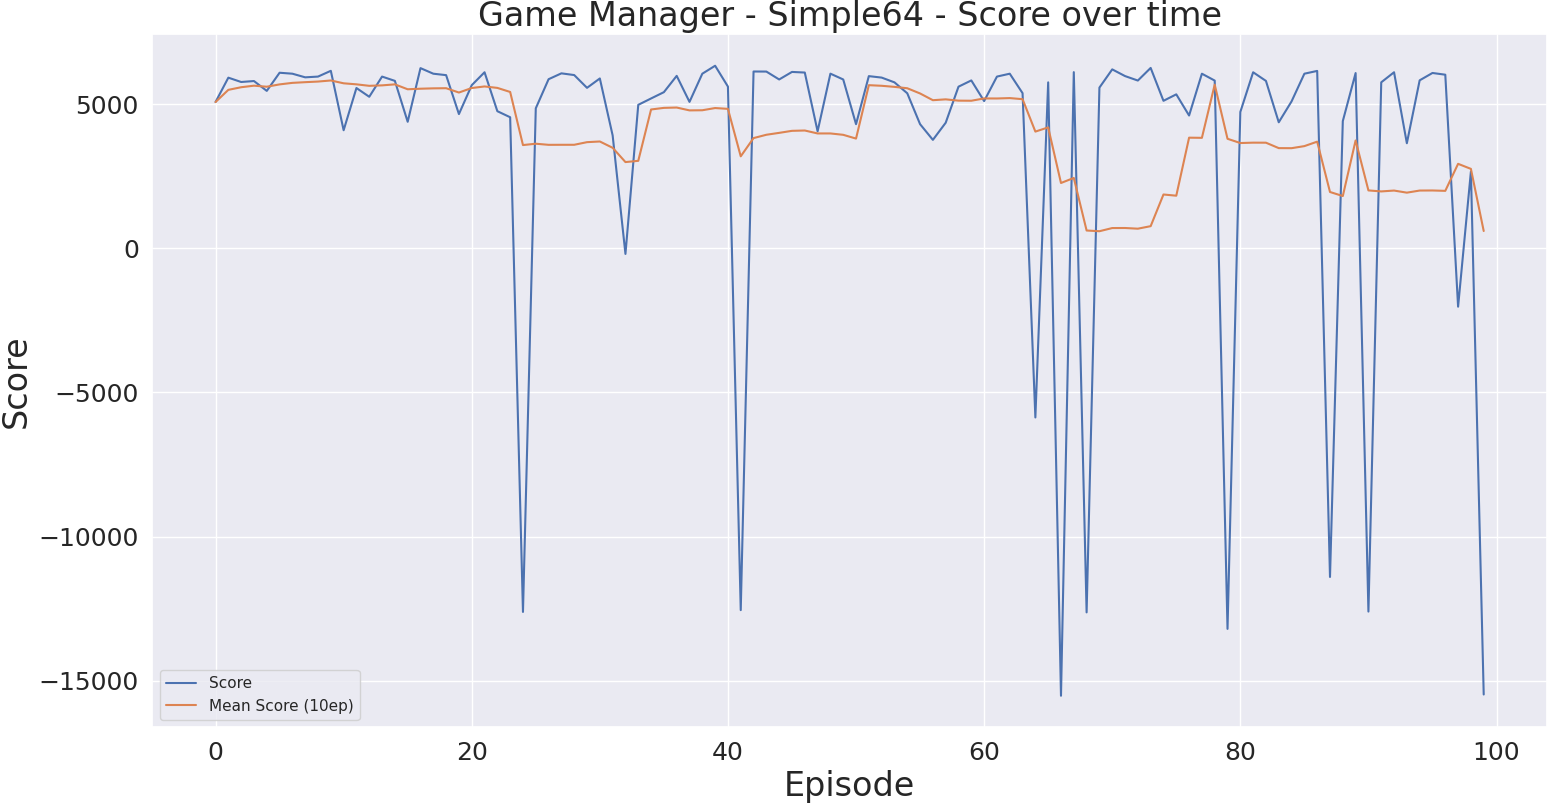
\includegraphics[width=1\textwidth]{figs/multi_dqn_game_manager/exploit/score.png}
        \caption{Hierarchical agent score}
    \end{subfigure}
    \hfill
    \begin{subfigure}[b]{0.48\textwidth}
        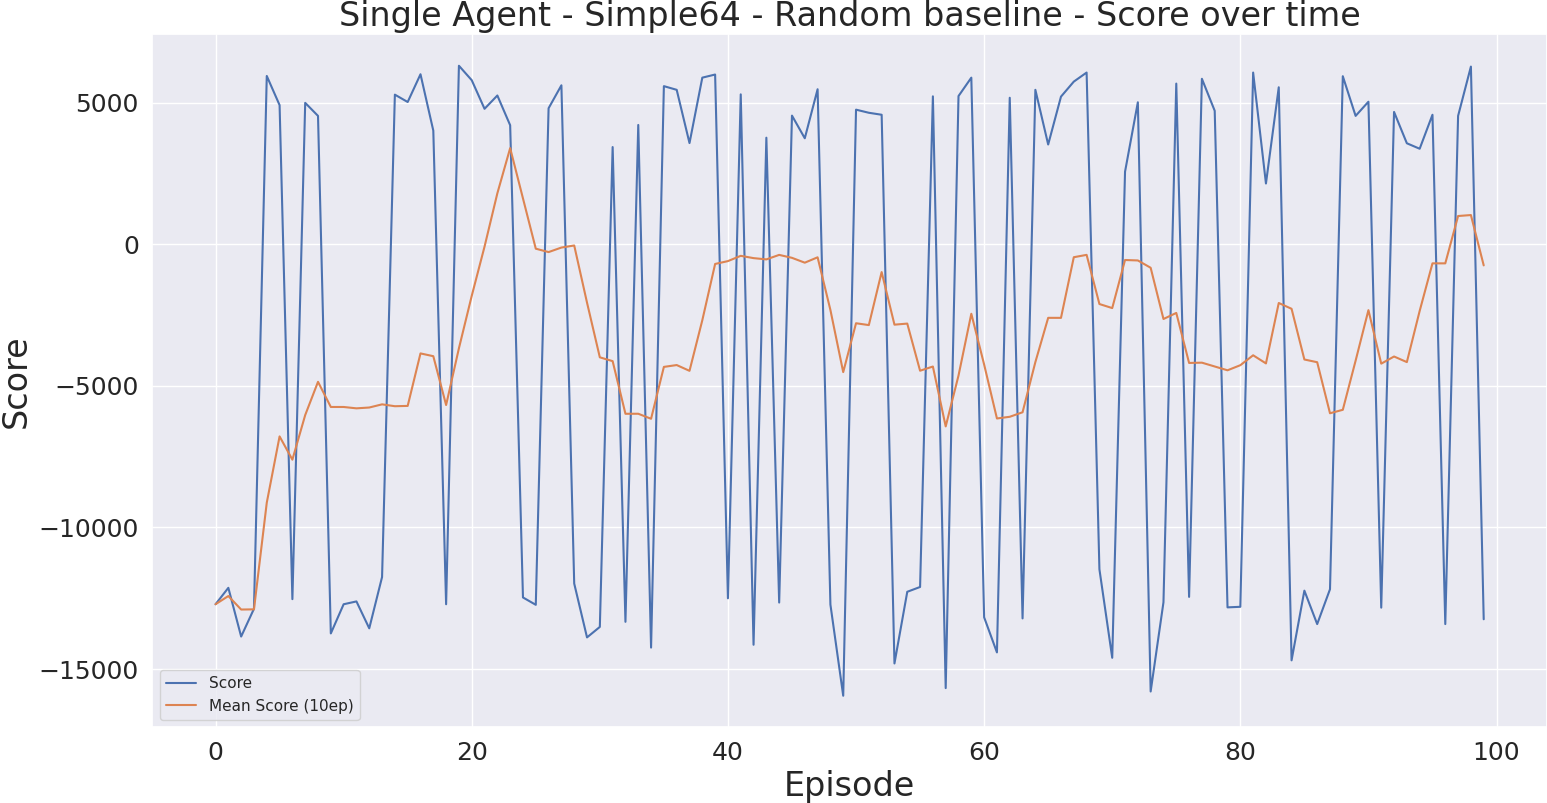
\includegraphics[width=1\textwidth]{figs/single_random/exploit/score.png}
        \caption{Random baseline score}
    \end{subfigure}
    \caption{Scores for hierarchical agent in \texttt{Simple64} map}
    \label{fig:hierarchical_Simple64_scores}
\end{figure}

\subsection{Single agent}

Finally, we have trained two instances of a RL agent to be used as the control for the performance and efficiency of the hierarchical agent. The first agent is meant to be as good as possible while being limited to the same training cost as the hierarchical agent. Conversely, the second is meant to match the performance of the hierarchical agent regardless of the training efficiency. Both agents haven been trained with the same environment and reward signal as the hierarchical agent.

The first agent uses a medium network (the same size as the networks of all hierarchical sub-agents) and has been trained for 52572 steps (130 episodes). For the second agent, we needed to upgrade to a large network to come close to the same performance as the hierarchical agent. It has been trained for 79768 steps (200 episodes). Figure \ref{fig:hierarchical_Simple64_scores} shows the scores obtained by both agents during exploitation compared to the ones obtained by a random agent.

\begin{figure}[t]
    \centering
    \begin{subfigure}[b]{0.48\textwidth}
        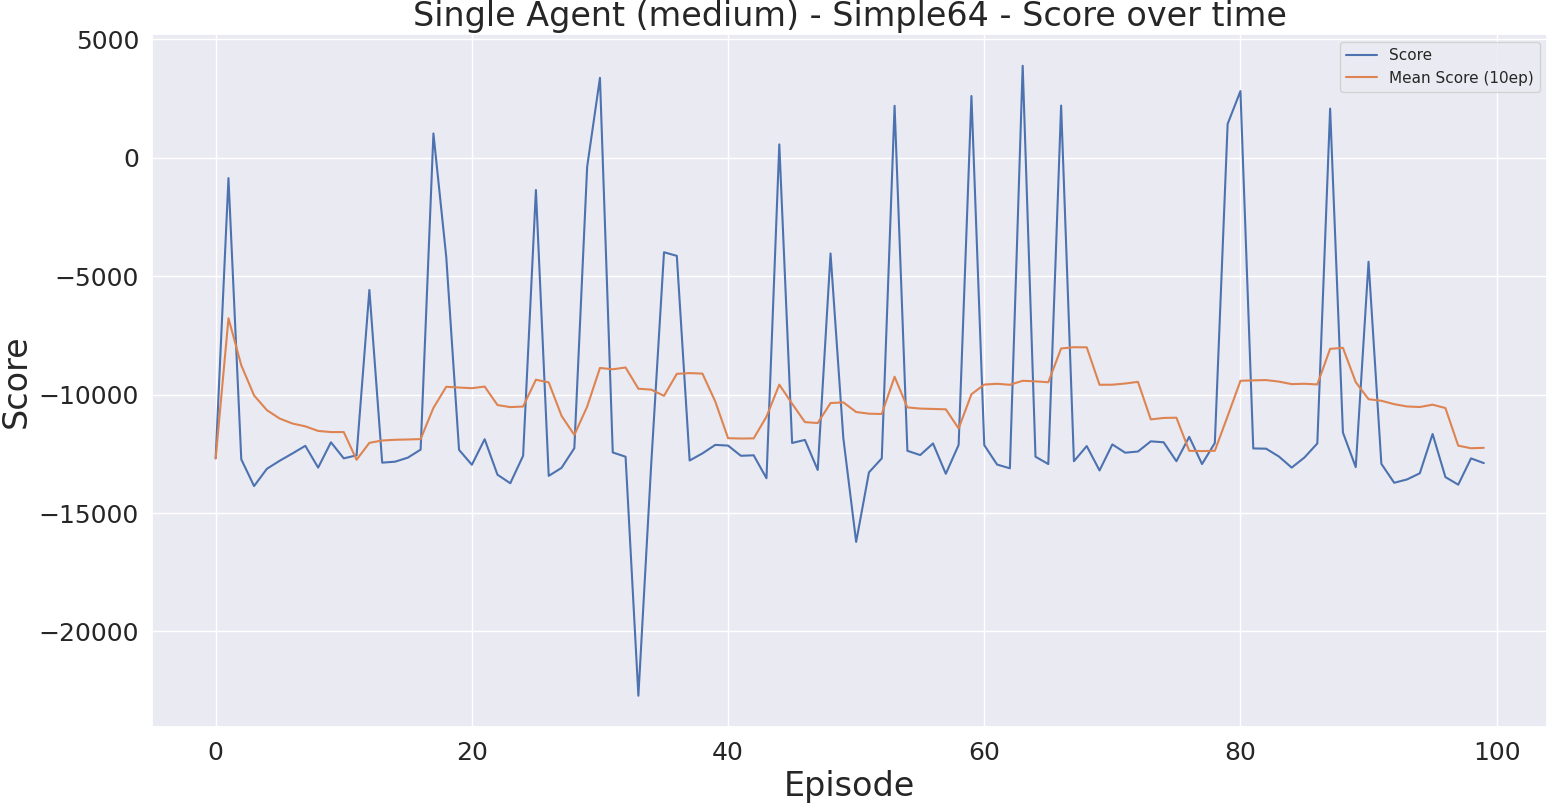
\includegraphics[width=1\textwidth]{figs/single_dqn_m_130/exploit/score.png}
        \caption{Single agent (medium) score}
    \end{subfigure}
    \hfill
    \begin{subfigure}[b]{0.48\textwidth}
        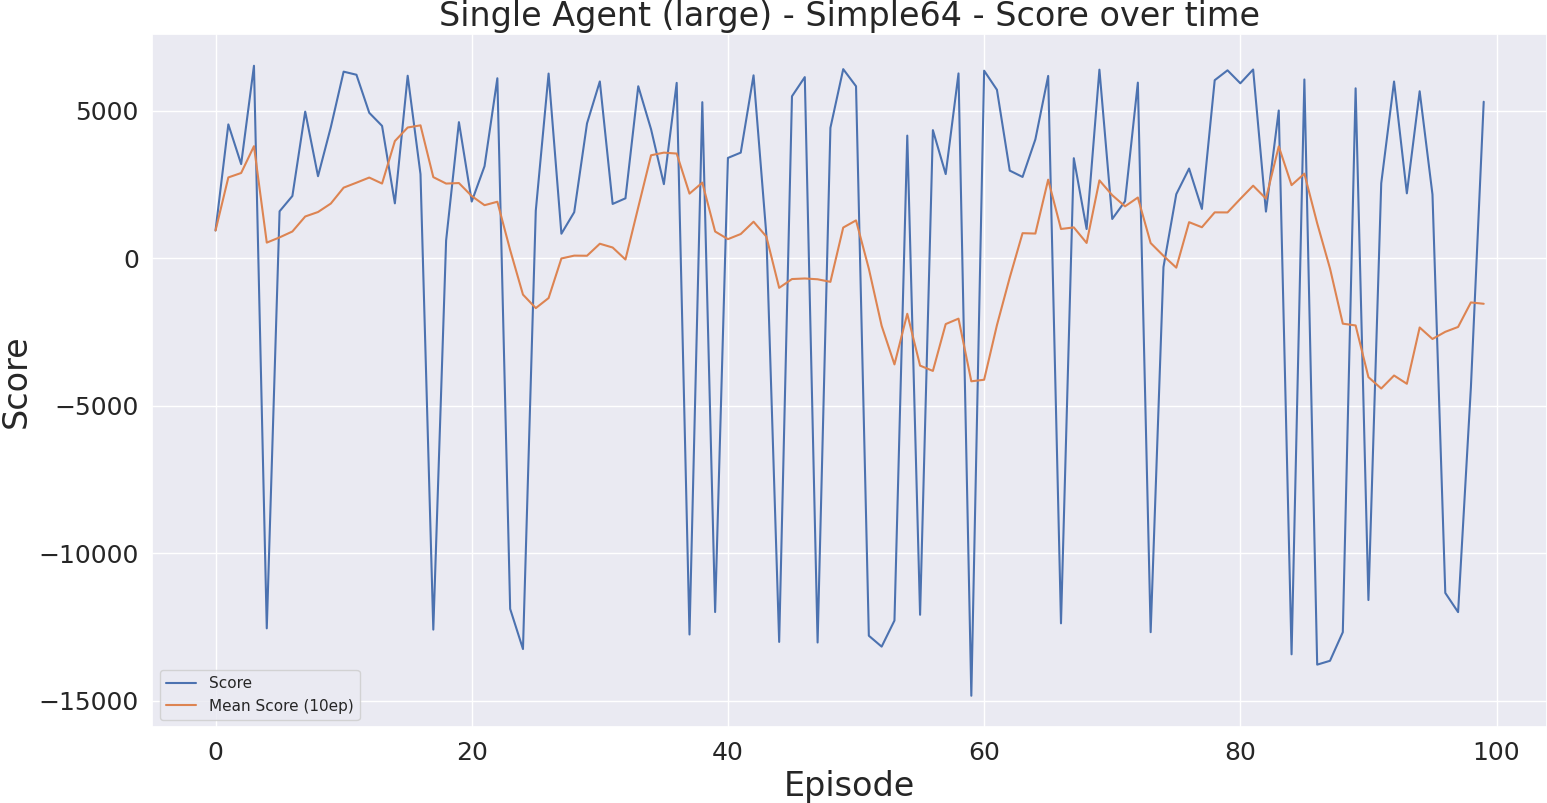
\includegraphics[width=1\textwidth]{figs/single_dqn_l_200/exploit/score.png}
        \caption{Single agent (large) score}
    \end{subfigure}
    \hfill
    \begin{subfigure}[b]{0.48\textwidth}
        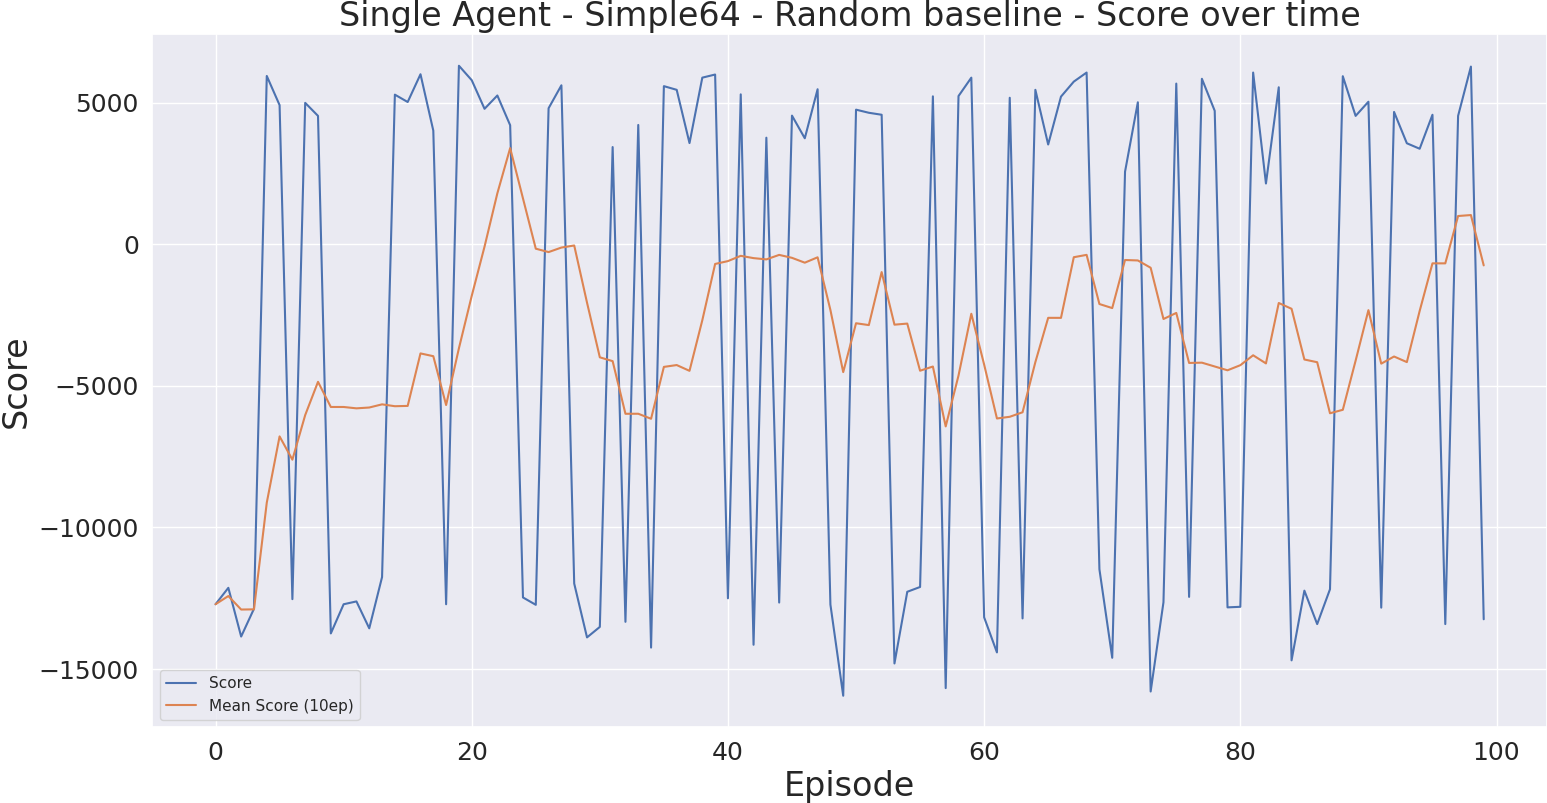
\includegraphics[width=1\textwidth]{figs/single_random/exploit/score.png}
        \caption{Random baseline score}
    \end{subfigure}
    \caption{Scores for single agent in \texttt{Simple64} map}
    \label{fig:single_Simple64_scores}
\end{figure}

\section{Results}

\begin{table}[t]
    \centering
    \begin{tabular}{ l|c l l l }
        & Performance & Energy (kW/h) & CO\textsubscript{2} emissions (kg) & FPOs \\
        \hline \hline
        Single agent M & \cellcolor{Maroon!25}$13$/$8$/$79$ ($13.00\%$) & \cellcolor{Dandelion!25}$0.09202$ & \cellcolor{Dandelion!25}$0.015547$ & \cellcolor{OliveGreen!25}$1.93\mathrm{e}12$ \\
        Single agent L & \cellcolor{Dandelion!25}$78$/$0$/$22$ ($78.00\%$) & \cellcolor{Maroon!25}$0.12199$ & \cellcolor{Maroon!25}$0.020814$ & \cellcolor{Maroon!25}$6.32\mathrm{e}12$ \\
        Hierarchical agent & \cellcolor{OliveGreen!25}$91$/$3$/$6$ ($91.00\%$) & \cellcolor{OliveGreen!25}$0.0889$ & \cellcolor{OliveGreen!25}$0.0150$ & \cellcolor{Dandelion!25}$2.02\mathrm{e}12$ \\
        \hline
        \quad Base manager & --- & $0.0207$ & $0.00349$ & $6.61\mathrm{e}11$ \\
        \quad Recruit manager & --- & $0.0225$ & $0.00380$ & $6.61\mathrm{e}11$ \\
        \quad Attack manager & --- & $0.00575$ & $0.000972$ & $2.26\mathrm{e}11$ \\
        \quad Game manager & --- & $0.0401$ & $0.00677$ & $4.71\mathrm{e}11$ \\
    \end{tabular}
    \caption{Results summary}
    \label{tab:results}
\end{table}

\begin{figure}[t]
    \centering
    \begin{subfigure}[b]{0.48\textwidth}
        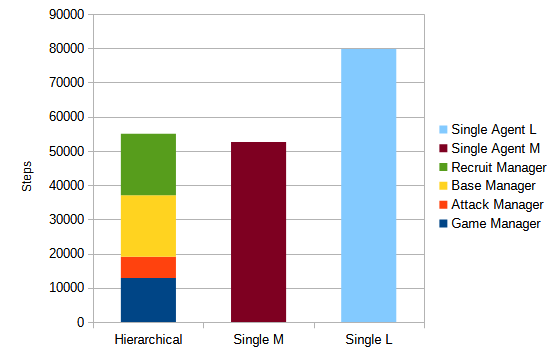
\includegraphics[width=1\textwidth]{figs/training_steps.png}
        \caption{Training steps}
    \end{subfigure}
    \hfill
    \begin{subfigure}[b]{0.48\textwidth}
        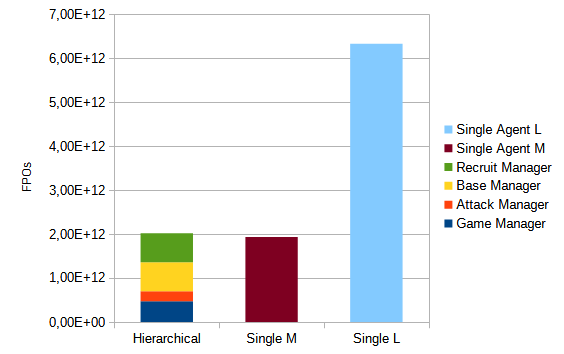
\includegraphics[width=1\textwidth]{figs/training_fpos.png}
        \caption{FPOs performed}
    \end{subfigure}
    \hfill
    \begin{subfigure}[b]{0.48\textwidth}
        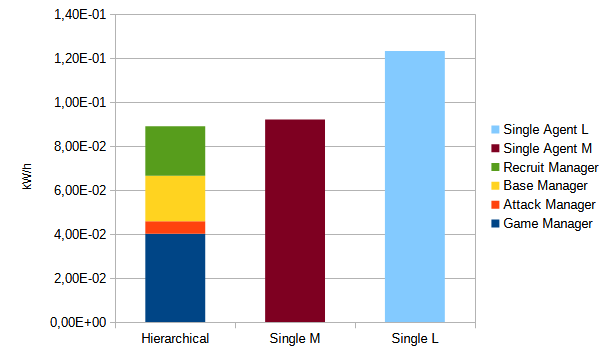
\includegraphics[width=1\textwidth]{figs/training_energy.png}
        \caption{Energy consumed}
    \end{subfigure}
    \hfill
    \begin{subfigure}[b]{0.48\textwidth}
        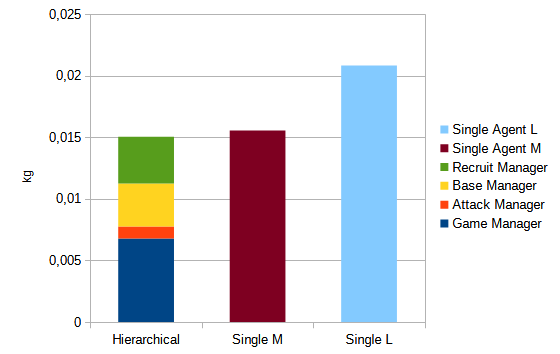
\includegraphics[width=1\textwidth]{figs/training_emissions.png}
        \caption{Carbon emissions}
    \end{subfigure}
    \caption{Training efficiency summary}
    \label{fig:results}
\end{figure}

Table \ref{tab:results} lists a summary of the results we have obtained, which are also visualized in figure \ref{fig:results}. After training was complete, we have measured the performance of the hierarchical agent and the two single agents by making them play 100 games in \texttt{Simple\_64} against a random agent. The hierarchical agent has achieved a 91\% win rate. The large single agent has had a worse, but still positive performance with a 78\% win rate, while the medium single agent has performed considerably worse than random, winning only 13\% of the games.

To measure the efficiency of the different agents during training, we have used the codecarbon\footnote{\url{https://codecarbon.io/}} Python library, which periodically measures the energy consumed by the hardware (CPU, GPU, etc.) and estimates the carbon emissions that would be generated by producing that amount of energy. However, due to hardware and operating system incompatibilities, codecarbon was not able to access the hardware on our setup, so all the measurements are a brute estimation based on a theoretical constant consumption. We include these values in the summary table for the sake of completeness, but they are not particularly accurate.

An alternative way to estimate the training cost of our models is to obtain the number of floating-point operations (FPOs) that are performed \cite{Schwartz:2019}. FPOs serve as an estimate of the work performed by a computational process, and using them as a measure has the advantage that it is independent of the hardware. While we can't obtain the exact number of FPOs performed during training, we can approximate them based on the size of the neural networks and the number of inferences and backpropagations executed.

For a completely connected neural network like the ones we use, the number of weights of each layer is equal to the product of the number of neurons in the layer and the number of neurons in the next layer. Our networks have 68 inputs and 15 outputs, except for the case of the hierarchical main agent, which has only 3 outputs, and the number of hidden layers and nodes depends on the sizes described in section \ref{sec:agent_structure}. The resulting amounts of weights for each network size are listed in table \ref{tab:weights}.

\begin{table}[h]
    \centering
    \begin{tabular}{ l|r r }
        Network size & Weights & Weights (game manager) \\
        \hline
        Medium & $35808$ & $35424$ \\
        Large & $77280$ & $76896$ \\
        Extra large & $225760$ & $225376$ \\
    \end{tabular}
    \caption{Number of weights of the neural networks}
    \label{tab:weights}
\end{table}

Following the DQN algorithm (algorithm \ref{alg:dqn2}), we can estimate the number of operations executed by each neural network of an agent. During training, the main network performs one inference on every step\footnote{Due to the $\epsilon$-greedy method, the agent doesn't actually calculate an action every step. However, even when taking that into account, the difference in the final calculation is four orders of magnitude smaller than the total result.} to select an action for the agent to take. Also every step, both the main and target network perform one inference for every experience in the update batch to estimate the q-value of the sample. Lastly, after the loss and gradients are calculated, the main network is updated through backpropagation. This results in the following formula to estimate the number of FPOs performed by the networks:

\begin{equation}
    \mathrm{FPO} \approx W \cdot (S + 2SJ + S) = 2WS(J+1)
\end{equation}

Where $W$ is the number of weights in the network, $S$ is the number of steps taken during training and $J$ is the learning batch size, which in our case is 512 for all agents.

After calculating the FPOs for each agent we see that training the single large agent involves three times more floating-point operations than the entire group of hierarchical agents.
\chapter{Conclusions and future work}
\label{chapter:conclusions}

\section{Conclusions}

The main goal of this project was to try to obtain experimental evidence supporting our hypothesis that, in an environment with a complex action and observation space, a hierarchical reinforcement learning model can generate agents with performance matching that of traditional models while producing less carbon emissions during training. To test this, we have expanded upon previous work from other students by improving the agents' implementation, increasing the action space while reducing the amount of pre-programmed logic, creating new environments, and improving the observations and reward signals.

We have trained a hierarchical agent and two single agents with different restrictions to compare their performance and training costs. The hierarchical agent was able to easily outperform an single agent with a considerably more costly training process, while the single agent limited to the same training cost as the hierarchical agent wasn't able to properly learn the environment, ending up with a performance worse than random. While the experimental phase wasn't exhaustive and we were limited by time constraints, our results lean heavily in favour of our original hypothesis.

When it comes to the training costs of the agents, we have observed two main benefits for the hierarchical model thanks to its use of sub-agents. The first is that, by training the sub-agents individually, their environments can be finely-tuned to their needs, leading to shorter learning times. We did this for our three sub-agents by creating custom training maps, but specially for the recruit manager for which we created two maps: one to facilitate exploration and a second to complete the training. The second benefit is that, since the sub-agents only need to learn simpler tasks (with smaller action and observation spaces), they can use smaller neural networks than single agents and train for smaller amounts of time. The combined benefit of smaller networks and reduced training time is such that, even when needing to create several smaller agents, the total compute cost is greatly reduced.

Looking back at the subgoals first defined in chapter \ref{chapter:introduction}, we can confidently say that we have achieved the first two: \textbf{Reducing built-in logic in actions} and \textbf{Improving the reward signal}. As for the third one, \textbf{Finding new subtasks}, we tried to find a part of the agent's existing game plan that could be handled by a new sub-agent, but were unable to find one that wasn't redundant or didn't involve dramatically increasing the number of tools that the agent can access, which would be beyond the scope of the project. The existing division of tasks between the sub-agents perfectly encapsulates the macro steps that the agents need to win the game.

\section{Future work}

Our work in this project is not definitive. With more time and resources it could be continued in several ways, examples of which are:

\begin{itemize}
    \item \textbf{Further expand the environment complexity.} Since we believe that an environment with a complex action and state space is one of the elements that allows a hierarchical agent to outshine a single agent, continuing the experiments in a more complex environment could help cement this idea. A way to achieve this could be expanding the actions that the agents can take (such as allowing them to repair damaged buildings, or complete structures left unfinished), increasing the number of units and resources that the agents have access to (introducing vespene gas and advanced units and structures), or even introducing one or both of the remaining playable races, either as opponents or for the agent to learn as well.
    \item \textbf{Improve reward signals.} Even though we have improved the reward signal for the \texttt{Simple\_64} map, we believe there is still room for improvement regarding the rewards of the sub-agents. To facilitate fine-tuning, we used short-term or immediate rewards when possible, but the rewards were not ideal for finding an optimal solution. Devising more accurate reward signals could go a long way to get more efficient policies.
    \item \textbf{Perform more extensive training.} Due to time limitations, the agents' training was not as thorough as could be desired. While we were unable to match the performance of the hierarchical agent using a single agent with a medium or large network, perhaps a better configuration or set of hyperparameters could yield better results. This also includes certain agent configurations such as the action frequency or the temporal extension of the hierarchical agent.
    \item \textbf{Experiment with different hierarchical strategies.} We have focused on the \textit{options} hierarchical strategy for this whole project, but other hierarchical methodologies could be tested to see if they provide the same efficiency benefits. An example would be Feudal HRL, in which a manager agent learns to define sub-tasks and rewards for its worker agents.
    \item \textbf{Improve efficiency measurements.} Lastly it would be beneficial to use hardware and software with better compatibility to be able to take accurate measurements of energy consumption with codecarbon, or to find an alternative way to obtain this data.
\end{itemize}

% \section{Results}

% Describe the results achieved using the previously described methodology.

% \section{Conclusions and future work}

% This section should include the following:

% \begin{itemize}
%     \item A description of the conclusions of the work.
%     \item A critical assessment of the degree of achievement of the initial goals.
%     \item A critical assessment of the schedule and methodology used in the project.
%     \item Considering the sustainability, diversity and ethical-social challenges linked to the project.
%     \item A discussion of topics for potential future work that have not been explored in this project.
% \end{itemize}

% \section{Glossary}

% Definition of the most relevant terms and acronyms used in this report.

% bibliography
\addcontentsline{toc}{chapter}{Bibliography}
\printbibliography
% \bibliographystyle{plain}
% \bibliography{references}

\appendix
% \appendixpage
\noappendicestocpagenum
\addappheadtotoc

\chapter{Algorithms}

\begin{algorithm}
\caption{Base DQN algorithm}
\label{alg:dqn1}
\begin{algorithmic}
    \ENSURE $Q_\theta \approx q_*$
    \STATE

    \STATE \textbf{Initialization:}
    \STATE Initialize $Q_\theta(s,a)$ with random weights $\theta$
    \STATE
    
    \FOR{each episode}
        \FOR{each step}
            \STATE Select an action $a$ for the current state $s$ following an greedy policy based on $Q_\theta(s,a)$
            \STATE Perform action $a$ and obtain the vector $(s,a,r,s^\prime)$
            \IF{episode ended}
                \STATE Set target value $y \gets r$
            \ELSE
                \STATE Set target value $y \gets r + \gamma \max_{a^\prime \in \mathcal{A}} Q_\theta(s^\prime,a^\prime)$
            \ENDIF
            \STATE Calculate the loss $\mathcal{L} = [Q_\theta(s,a)-y]^2$
            \STATE Update $Q_\theta$ with backpropagation and gradient descent minimizing the loss
        \ENDFOR
    \ENDFOR
    \STATE
    
    \RETURN $Q_\theta$
\end{algorithmic}
\end{algorithm}


\begin{algorithm}
\caption{Final DQN algorithm}
\label{alg:dqn2}
\begin{algorithmic}
    \REQUIRE $N, J$
    \ENSURE $Q_\theta \approx q_*$
    \STATE

    \STATE \textbf{Initialization:}
    \STATE Initialize $Q_\theta(s,a)$ with random weights $\theta$
    \STATE Initialize $\hat{Q}_{\theta^-}(s,a)$ with weights $\theta^- = \theta$
    \STATE Initialize replay buffer $D$
    \STATE
    
    \FOR{each episode}
        \FOR{each step}
            \STATE Select an action $a$ for the current state $s$ following an $\epsilon$-greedy policy based on $Q_\theta(s,a)$
            \STATE Perform action $a$ and store the vector $(s,a,r,s^\prime)$ in the replay buffer $D$
            \STATE Select a random subset $(s_j,a_j,r_j,s^\prime_j)$ of $J$ experiences from the replay buffer $D$
            \FOR{each transition $j$}
                \IF{episode ended}
                    \STATE Set target value $y_j \gets r_j$
                \ELSE
                    \STATE Set target value $y_j \gets r_j + \gamma \max_{a^\prime_j \in \mathcal{A}} \hat{Q}_{\theta^-}(s^\prime_j,a^\prime_j)$
                \ENDIF
            \ENDFOR
            \STATE Calculate the loss $\mathcal{L} \gets \frac{1}{J} \sum^{J-1}_{j=0} [Q_\theta(s_j,a_j) - y_j]^2$
            \STATE Update $Q_\theta$ with backpropagation and gradient descent minimizing the loss
            \STATE Every $N$ iterations, clone the weights from $Q_\theta$ to $\hat{Q}_{\theta^-}$: $\theta^- \gets \theta$
            \STATE Decrement $\epsilon$
        \ENDFOR
    \ENDFOR
    \STATE

    \RETURN $Q_\theta$
\end{algorithmic}
\end{algorithm}
\chapter{Observation fields}
\label{app:observation}

\subsubsection*{Relating to actions}
\begin{description}
    \item[\texttt{can\_harvest\_minerals}] $1$ if the agent can take the \texttt{HARVEST\_MINERALS} action, $0$ otherwise.
    \item[\texttt{can\_recruit\_worker\_0}] $1$ if the agent can take the \texttt{RECRUIT\_SCV\_0} action, $0$ otherwise.
    \item[\texttt{can\_recruit\_worker\_1}] $1$ if the agent can take the \texttt{RECRUIT\_SCV\_1} action, $0$ otherwise.
    \item[\texttt{can\_recruit\_worker\_2}] $1$ if the agent can take the \texttt{RECRUIT\_SCV\_2} action, $0$ otherwise.
    \item[\texttt{can\_build\_supply\_depot}] $1$ if the agent can take the \texttt{BUILD\_SUPPLY\_DEPOT} action, $0$ otherwise.
    \item[\texttt{can\_build\_command\_center}] $1$ if the agent can take the \texttt{BUILD\_COMMAND\_CENTER} action, $0$ otherwise.
    \item[\texttt{can\_build\_barracks}] $1$ if the agent can take the \texttt{BUILD\_BARRACKS} action, $0$ otherwise.
    \item[\texttt{can\_recruit\_marine}] $1$ if the agent can take the \texttt{RECRUIT\_MARINE} action, $0$ otherwise.
    \item[\texttt{can\_attack\_closest\_buildings}] $1$ if the agent can take the \texttt{ATTACK\_CLOSEST\_BUILDING} action, $0$ otherwise.
    \item[\texttt{can\_attack\_closest\_workers}] $1$ if the agent can take the \texttt{ATTACK\_CLOSEST\_WORKER} action, $0$ otherwise.
    \item[\texttt{can\_attack\_closest\_army}] $1$ if the agent can take the \texttt{ATTACK\_CLOSEST\_ARMY} action, $0$ otherwise.
    \item[\texttt{can\_attack\_buildings}] $1$ if the agent can take the \texttt{ATTACK\_BUILDINGS} action, $0$ otherwise.
    \item[\texttt{can\_attack\_workers}] $1$ if the agent can take the \texttt{ATTACK\_WORKERS} action, $0$ otherwise.
    \item[\texttt{can\_attack\_army}] $1$ if the agent can take the \texttt{ATTACK\_ARMY} action, $0$ otherwise.
\end{description}

\subsubsection*{Relating to structures}
\begin{description}
    \item[\texttt{num\_command\_centers}] Number of Command Centers the agent controls (includes Command Centers being build).
    \item[\texttt{num\_completed\_command\_centers}] Number of finished Command Centers the agent controls.
    \item[\texttt{max\_command\_centers}] Maximum number of commands centers the agent can have at a time (as configured for the current map).
    \item[\texttt{pct\_command\_centers}] Number of Command Centers divided by maximum number of commands centers.
    \item[\texttt{command\_center\_0\_order\_length}] Number of workers being build in first Command Center.
    \item[\texttt{command\_center\_0\_num\_workers}] Number of workers harvesting minerals to first Command Center.
    \item[\texttt{command\_center\_1\_order\_length}] Number of workers being build in second Command Center.
    \item[\texttt{command\_center\_1\_num\_workers}] Number of workers harvesting minerals to second Command Center.
    \item[\texttt{command\_center\_2\_order\_length}] Number of workers being build in third Command Center.
    \item[\texttt{command\_center\_2\_num\_workers}] Number of workers harvesting minerals to third Command Center.
    \item[\texttt{num\_supply\_depots}] Number of Supply Depots the agent controls (includes Supply Depots being build).
    \item[\texttt{num\_completed\_supply\_depots}] Number of finished Supply Depots the agent controls.
    \item[\texttt{max\_supply\_depots}] Maximum number of Supply Depots the agent can have at a time (as configured for the current map).
    \item[\texttt{pct\_supply\_depots}] Number of Supply Depots divided by maximum number of Supply Depots.
    \item[\texttt{num\_barracks}] Number of Barracks the agent controls (includes Barracks being build).
    \item[\texttt{num\_completed\_barracks}] Number of finished Barracks the agent controls.
    \item[\texttt{max\_barracks}] Maximum number of Barracks the agent can have at a time (as configured for the current map).
    \item[\texttt{pct\_barracks}] Number of Barracks divided by maximum number of Barracks.
    \item[\texttt{barracks\_used\_queue\_length}] Number of Marines being build in all Barracks.
    \item[\texttt{barracks\_free\_queue\_length}] Number of that can be queued to build in all Barracks.
\end{description}

\subsubsection*{Relating to units}
\begin{description}
    \item[\texttt{num\_workers}] Number of worker units the agent controls.
    \item[\texttt{num\_idle\_workers}] Number of workers that are idle.
    \item[\texttt{pct\_idle\_workers}] Ratio of workers that are idle.
    \item[\texttt{num\_mineral\_harvesters}] Number of workers that are harvesting minerals.
    \item[\texttt{pct\_mineral\_harvesters}] Ratio of workers that are harvesting minerals.
    \item[\texttt{num\_marines}] Number of Marines the agent controls.
    \item[\texttt{num\_idle\_marines}] Number of Marines that are idle.
    \item[\texttt{pct\_idle\_marines}] Ratio of Marines that are idle.
    \item[\texttt{total\_army\_health}] Total health of all Marines.
    \item[\texttt{dist\_marine\_avg\_to\_army\_avg}] Distance from average position of all Marines to average position of all enemy Marines.
    \item[\texttt{dist\_marine\_avg\_to\_worker\_avg}] Distance from average position of all Marines to average position of all enemy workers.
    \item[\texttt{dist\_marine\_avg\_to\_building\_avg}] Distance from average position of all Marines to average position of all enemy structures.
    \item[\texttt{dist\_marine\_avg\_to\_closest\_army}] Shortest distance from average position of all Marines to any enemy Marine.
    \item[\texttt{dist\_marine\_avg\_to\_closest\_worker}] Shortest distance from average position of all Marines to any enemy worker.
    \item[\texttt{dist\_marine\_avg\_to\_closest\_building}] Shortest distance from average position of all Marines to any enemy structure.
\end{description}

\subsubsection*{Relating to resources}
\begin{description}
    \item[\texttt{free\_supply}] Available supply resource.
    \item[\texttt{minerals}] Mineral resource count.
    \item[\texttt{collection\_rate\_minerals}] Mineral collection rate in minerals per second.
\end{description}

\subsubsection*{Relating to score}
\begin{description}
    \item[\texttt{score\_cumulative\_score}] Game-calculated overall score.
    \item[\texttt{score\_cumulative\_total\_value\_units}] Mineral value of all units owned.
    \item[\texttt{score\_cumulative\_total\_value\_structures}] Mineral value of all structures owned.
    \item[\texttt{score\_cumulative\_killed\_value\_units}] Mineral value of all units killed.
    \item[\texttt{score\_cumulative\_killed\_value\_structures}] Mineral value of all structures destroyed.
    \item[\texttt{score\_food\_used\_army}] Total supply used in army units (marines).
    \item[\texttt{score\_food\_used\_economy}] Total supply used in economy units (workers).
    \item[\texttt{score\_used\_minerals\_army}] Total minerals used in army units (marines).
    \item[\texttt{score\_used\_minerals\_economy}] Total minerals used in economy units and structures (command centers, workers and Supply Depots).
    \item[\texttt{score\_used\_minerals\_technology}] Total minerals used in technology structures (barracks).
    \item[\texttt{damage\_dealt\_delta}] Damage dealt since last observation.
    \item[\texttt{damage\_taken\_delta}] Damage received since last observation.
\end{description}

\subsubsection*{Relating to neural units}
\begin{description}
    \item[\texttt{num\_minerals}] Number of mineral deposits in the map.
\end{description}

\subsubsection*{Relating to enemy units}
\begin{description}
    \item[\texttt{enemy\_total\_building\_health}] Total health of enemy buildings.
    \item[\texttt{enemy\_total\_worker\_health}] Total health of enemy workers.
    \item[\texttt{enemy\_total\_army\_health}] Total health of enemy Marines.
\end{description}
\chapter{Agents training stats}
\label{app:stats}

\subsubsection*{Relating to actions}


% List of sections that are too long to be included in the body of the report and that are self-contained.

\end{document}